\documentclass[english,bibfile=bibliography]{algotemplate/thesis}

\usepackage{tikz}
\usetikzlibrary{arrows.meta,positioning}

% ------------------------------------------ Title page ------------------------
\title{Time-Dependent Decision Making in Heuristic Chess Search}
\type{Bachelor Thesis}
\author{Marvin Becker}
\studentno{01/1365135}
\group{Algorithmics}
\department{Computer and Information Science}
\institute{University of Konstanz}
\advisor{Prof.~Dr.~Sabine Storandt}
\reviewer{Prof.~Dr.~Sabine Storandt\\ & Prof.~Dr.~Michael Grossniklaus}
\date{2026-09-01}
% ------------------------------------------------------------------------------

% ------------------------------------------ Abstract --------------------------
\begin{abstract}
Chess engines rely on heuristic search to cope with the exponential growth of the
game tree, and under a clock the decisive question is how much additional
computation is actually worth. This thesis investigates where the sweet spot
between invested time and decision quality lies: how much extra search time
translates into better moves, and from which point on further computation no
longer changes the decision.

A complete engine is implemented from scratch in \texttt{C++} on a classical
mailbox board representation, combining alpha-beta search, transposition tables,
quiescence search, heuristic move ordering and a two-stage time management. On
this baseline three established refinements are implemented and evaluated:
Principal Variation Search, null-move pruning, and the reuse of previous search
trees through a persistent transposition table. The evaluation uses a suite of
309 positions across budgets from 10\,ms to 5\,s, with move quality scored as
centipawn loss against a strong reference engine, and a 400-game match against a
strength-limited opponent, won by $205 \pm 38$ Elo, as an external check.

All three refinements deliver depth as intended: at a one-second budget null-move
pruning gains a full ply, Principal Variation Search $0.23$ and tree reuse $0.25$
ply, each with $95\,\%$ confidence intervals excluding zero. For none of them
could a corresponding improvement in move quality be detected. Two observations
explain this. Decisions settle early, as three quarters of all positions have
fixed their move by the depth the engine already reaches. And the residual error
is highly concentrated: the median centipawn loss is $2$ while the mean is $52$,
with fifteen positions accounting for nearly half of that mean. These are
predominantly sparse endgames, and they respond to additional depth far more
weakly than the rest of the suite.

The value of additional computation is therefore highly heterogeneous across
positions. Under an explicit criterion, no further improvement of typical move
quality is detectable beyond roughly one second per move on this suite, while
average quality keeps falling through that difficult minority. This is consistent
with limitations of the static evaluation contributing substantially to the
residual error.
\end{abstract}
% ---------------
% ------------------------------------------------------------------------------

% --------------------------------- Document / Main Content --------------------
\begin{document}

\section{Introduction}
\label{sec:introduction}
% Motivation, problem statement, goals, research question

Chess has long been regarded as a canonical benchmark problem in artificial
intelligence and algorithm engineering. Despite its simple and fully specified
rules, the game exhibits an enormous search space caused by its high branching
factor and strategic depth. As a consequence, exhaustive search of the complete
game tree is computationally infeasible, even with modern hardware, and chess
engines must rely on heuristic search techniques to make strong decisions under
limited computational resources.

At the core of most classical chess engines lies a depth-limited game tree
search based on Minimax or Negamax, enhanced by Alpha-Beta pruning. Over the
years, a variety of improvements have been proposed to increase search
efficiency, including iterative deepening, transposition tables, quiescence
search, and heuristic move ordering. Among these techniques, iterative
deepening has become a standard approach, particularly in time-controlled
settings, as it allows the engine to gradually refine its decision while always
maintaining a valid best move.

The primary motivation of this work is to investigate the effectiveness of
iterative deepening when operating under explicit time constraints. While
iterative deepening is widely used in practice, it repeatedly re-searches the
game tree at increasing depths, which raises the question of how much efficiency
is lost compared to a fixed-depth search when the available time is limited.
This leads to the central research question of this thesis:

\emph{To what extent does the effectiveness of iterative deepening degrade under
strict time constraints, and how well can modern search heuristics compensate
for this overhead?}

To address this question, a complete chess engine is implemented from scratch in
\texttt{C++}. The engine deliberately employs a classical mailbox-based board
representation rather than highly optimized bitboard techniques. This design
choice emphasizes architectural clarity, ease of reasoning, and suitability for
academic analysis, allowing the impact of search algorithms and time management
to be studied in isolation from low-level optimizations.

The implemented engine integrates a Negamax search with Alpha-Beta pruning,
iterative deepening, quiescence search, transposition tables, and heuristic move
ordering. A dedicated time management module supports multiple search modes,
including fixed depth, fixed time, node-limited, and infinite search, following
the UCI protocol. In particular, a two-stage time budget with soft and hard
deadlines is used to control the interaction between iterative deepening and
time constraints.

The contribution of this work is twofold. First, it provides a clean and modular
implementation of a classical chess engine that serves as a transparent
experimental platform. Second, it presents an empirical evaluation of
iterative deepening under time constraints, analyzing its impact on search
depth, node counts, and move stability. The results aim to shed light on the
practical trade-offs between search efficiency and decision quality in
time-controlled chess engines.

The remainder of this report is structured as follows. \cref{sec:related_work}
discusses relevant prior work in computer chess and game tree search.
\cref{sec:preliminaries} introduces the necessary theoretical background.
The architecture and implementation of the engine are described in
\cref{sec:architecture} and \cref{sec:search}. The evaluation function and time
management are detailed in subsequent sections, followed by an experimental
evaluation and a discussion of the results. Finally, conclusions and directions
for future work are presented.

\cleardoublepage
\section{Related Work}
\label{sec:related_work}
% Classical chess engines, alpha-beta, iterative deepening, time control

The problem of efficient search in chess engines has been studied extensively
over several decades~\cite{marsland1986review}. Early approaches were based on the Minimax algorithm,
which provides an optimal decision strategy under the assumption of perfect
play~\cite{yannakakis2018artificial}. However, due to the exponential growth of the game tree, Minimax quickly becomes infeasible even at moderate depths.

Alpha-Beta pruning was introduced as a major improvement over plain Minimax,
allowing large parts of the search tree to be pruned without affecting the
correctness of the result~\cite{knuth1975alphabeta}. Subsequent work showed that
the effectiveness of Alpha-Beta pruning depends crucially on the order in which
moves are explored. With perfect move ordering, the effective branching factor can be reduced dramatically, enabling much deeper searches within the same computational budget~\cite{marsland1986review}.

Iterative deepening~\cite{korf1985iterative} has emerged as a standard technique to improve move ordering
and to support time-controlled search. By repeatedly searching the game tree with
increasing depth limits, iterative deepening ensures that a valid best move is
always available while simultaneously refining the move ordering for deeper
iterations. Despite the apparent redundancy caused by re-searching parts of the
tree, it has been shown that the overhead is often compensated by improved
pruning efficiency~\cite{marsland1986review}.

A detailed analysis of Alpha-Beta pruning efficiency in chess engines is
presented by Nair~\cite{nair_improving_ab}. The paper investigates how different
move ordering heuristics and search enhancements affect the pruning behavior of
Alpha-Beta search. In particular, it highlights the strong interaction between
iterative deepening, transposition tables, and heuristic move ordering. The
results indicate that improved move ordering can significantly reduce the number
of explored nodes, even when additional search iterations are introduced.

Building directly on the observation that Alpha-Beta search is most effective
with strong move ordering, several refinements of the basic algorithm have been
proposed. Pearl introduced the Scout algorithm, which verifies promising moves with
minimal-window tests before evaluating them exactly~\cite{pearl1980scout}.
Marsland and Campbell transferred this idea to the Alpha-Beta framework in the
form of Principal Variation Search~\cite{marsland1982parallel}, and Reinefeld
later refined it into NegaScout, analyzing the conditions under which the
additional re-searches pay off~\cite{reinefeld1983negascout}. PVS is
particularly effective in combination with iterative deepening and
transposition tables, since both increase the probability that the first move
searched is indeed the best one~\cite{marsland1986review}.

Transposition tables have further improved search efficiency by allowing engines
to reuse previously computed results for positions reached via different move
orders~\cite{zobrist1970hashing}. By storing evaluations together with depth
information and bound types, transposition tables enable both direct cutoffs and
enhanced move ordering. Their effectiveness is especially pronounced in
combination with iterative deepening, where information from earlier iterations
can be reused almost immediately~\cite{warnock1988search}. Beyond single search
invocations, a persistent transposition table also allows information to be
carried over from one move to the next, effectively resuming previously
explored search trees instead of recomputing them from scratch.

Quiescence search addresses another well-known limitation of depth-limited
search, commonly referred to as the horizon effect. By extending the search in
tactically unstable positions, quiescence search produces more reliable
evaluations and has become a standard component of classical chess
engines~\cite{marsland1986review}.

Beyond exact pruning, engines also employ heuristic forward pruning, which
discards subtrees without proving them irrelevant. The most widely used variant
is null-move pruning: if passing a turn still leaves the position good enough to
cause a cutoff, the subtree is assumed to be safe to skip. The null move as a
search device is considerably older than this application of it, but the
recursive form with depth reduction that engines use today was established
experimentally by Goetsch and Campbell~\cite{goetsch1990experiments}. Unlike
Alpha-Beta this is not value-preserving, so it trades a small risk of overlooking
a line for a substantially smaller tree.

Closest to the question of this thesis is the work on how additional search
actually pays off. Junghanns et al.~\cite{junghanns1997diminishing} studied
diminishing returns in self-play and found the winning percentage per additional
ply to decrease with depth. They also report that this decrease is not visible
throughout: the high error rate of chess programs hides the effect for search
depths through nine plies, which is precisely the range in which the engine
studied here operates. Ferreira~\cite{ferreira2013impact} approached the
same relationship from the other direction and related search depth to Elo,
reporting gains per ply that shrink as depth grows.

These studies establish that the returns of additional search diminish, but they
measure it through game outcomes between engines of differing depth. What they do
not address is where the returns diminish \emph{within a single engine under a
clock}, at which depth its decisions stop changing, and which positions cause the
remaining error. This thesis takes that perspective: instead of relating depth to
playing strength, it relates the time budget to the quality of the individual
decision on a fixed set of positions, and separates the positions in which
additional search still changes the decision from those in which it does not.

While modern state-of-the-art engines incorporate additional techniques such as
bitboards, evaluation learning, and neural networks~\cite{silver2018alphazero},
the classical search principles discussed above remain fundamental. This work
builds upon these established ideas.

\cleardoublepage
\section{Preliminaries}
\label{sec:preliminaries}

This section introduces the fundamental concepts and definitions required to
understand the remainder of this thesis. It establishes the formal game-theoretic
model of chess, derives the associated search problem, and motivates the use of
heuristic evaluation and time-constrained search. All concepts presented in this
section are standard in the field of computer chess and provide a common basis
for the subsequent chapters.

\subsection{Chess as a Game-Theoretic Model}

Chess is modeled as a deterministic, two-player, zero-sum game with perfect
information. At any point in time, the complete game state is fully observable
to both players, and no randomness is involved in the game mechanics.

A game state consists of a board configuration together with additional state
information such as the side to move, castling rights, and en-passant
availability. Players alternate turns by selecting legal moves, and the game
terminates in a win, loss, or draw according to the rules of chess.

More formally, let $\mathcal{T} = \{\text{pawn}, \text{knight}, \text{bishop},
\text{rook}, \text{queen}, \text{king}\}$ denote the set of piece types and
$\mathcal{C} = \{\text{white}, \text{black}\}$ the set of colours. A piece is then
an element of $\mathcal{F} = \mathcal{T} \times \mathcal{C}$, and the placement of
pieces on the board is described by a mapping
\[
b : \{1, \dots, 8\}^2 \rightarrow \mathcal{F} \cup \{\varnothing\},
\]
which assigns to each square either a piece or the empty symbol $\varnothing$. A
complete game state $s = (b, t, r, e)$ additionally comprises the side to move
$t \in \mathcal{C}$, the castling rights $r$, and the en-passant target $e$, both
of which depend on the movement history rather than on the current placement
alone. The set of all legal states is denoted by $\mathcal{S}$.

The rules of chess induce a transition relation
$\delta \subseteq \mathcal{S} \times \mathcal{S}$, where $(s, s') \in \delta$ if
and only if $s'$ can be reached from $s$ by exactly one legal move. This relation
defines a directed graph $G = (\mathcal{S}, \delta)$ in which each node is a legal
position and each edge is a legal move. A state $s$ is \emph{terminal} if it has
no outgoing edges, as in checkmate or stalemate, or if it is declared drawn by
the rules of chess.

For decision making, the graph $G$ is unrolled into a game tree rooted at the
current position. Each level of the tree corresponds to one ply, and the number of
nodes per level is governed by the branching factor of chess, which amounts to
around $30$ available actions per position~\cite{yannakakis2018artificial}.

\subsection{Search Problem Formulation}

Given a current position, the task of a chess engine is to select a legal move
that maximizes the expected outcome under the assumption of optimal play by both
sides. In the classical formulation, the possible outcomes are associated with
numerical values, for example $+1$ for a win, $0$ for a draw, and $-1$ for a
loss.

This decision problem is commonly formulated as a game tree search problem, in
which the engine explores a subset of the game tree to estimate the value of
available moves. The root of the tree corresponds to the current position, while
internal nodes represent positions reachable through sequences of legal moves.

With that branching factor the tree grows exponentially with depth, so evaluating
all reachable positions is computationally infeasible even for moderate depths.
Consequently, the search must be limited by depth,
time, or other computational resources. This limitation introduces approximation:
the engine can no longer guarantee optimal play, but instead aims to select the
best move according to the information explored within the available budget.

The quality of a move selected by a chess engine therefore depends on two main
factors: the effectiveness of the search algorithm in selecting which parts of
the tree to explore, and the accuracy of the evaluation function used to estimate
the value of positions at the search frontier.

\subsection{Minimax, Negamax, Quiescence and Alpha-Beta Pruning}
\label{subsec:minimax_alphabeta}

The classic algorithmic solution to game tree search in two-player zero-sum
games with perfect information is the Minimax algorithm. Minimax assumes that
one player aims to maximize the evaluation value of a position, while the
opponent aims to minimize it. Terminal positions are assigned fixed values
corresponding to win, loss, or draw, while non-terminal leaf positions are
evaluated heuristically.

The algorithm explores the game tree recursively and propagates values from the
leaves toward the root by alternating between maximization and minimization
steps. A detailed introduction to Minimax can be found in standard textbooks on
artificial intelligence in games, such as Yannakakis and
Togelius~\cite{yannakakis2018artificial}.

\paragraph{Negamax Formulation}
In zero-sum games, the Minimax algorithm can be simplified using the Negamax
formulation. Instead of explicitly distinguishing between maximizing and
minimizing players, Negamax expresses all evaluations from the perspective of the
side to move. The value of a position is defined as the negation of the value
obtained by the opponent after making a move.

This formulation exploits the symmetry of \emph{two-player} zero-sum games, in
which one side's gain is exactly the other's loss, so that a single score suffices
if it is always read from the perspective of the side to move. It allows the
search to be implemented using a single recursive procedure. Negamax is
functionally equivalent to Minimax but leads to more compact and uniform code,
which is why it is widely used in practical chess engines.

\paragraph{Quiescence Search}
Depth-limited game tree search combined with static evaluation functions suffers
from a well-known problem referred to as the \emph{horizon effect}. Tactical
events such as captures, checks, or promotions may occur just beyond the search
depth and are therefore not accounted for by the evaluation function. As a
result, the engine may incorrectly assess positions as stable even though
significant tactical changes are imminent.

Quiescence search is a standard technique to solve this problem. Instead of
evaluating a position immediately when the nominal search depth is reached, the
search is selectively extended in positions that are considered tactically
unstable. Typically, only forcing moves such as captures or checking moves are
explored, while quiet moves are excluded.

The goal of quiescence search is to reach a \emph{quiescent} position, that is, a
position in which no immediate tactical exchanges are available and the static
evaluation is therefore more reliable. Once such a position is reached, the
evaluation function is applied and the resulting score is propagated back up the
search tree.

\cref{fig:horizon} shows why a fixed depth limit is not merely imprecise but can
be actively misleading. An exchange of pieces unfolds over several plies, and its
intermediate states are wildly unbalanced: after one side has captured but before
the recapture, the position looks winning by a whole piece. A search that stops
exactly at that moment reports this intermediate state as the final one. The
error is not small and random but large and systematic, since it always favors
the side that captured last. This is also the reason a purely depth-based
comparison of search algorithms is fragile without quiescence search, as one
additional ply can invert the sign of the evaluation.

\begin{figure}[ht]
\centering
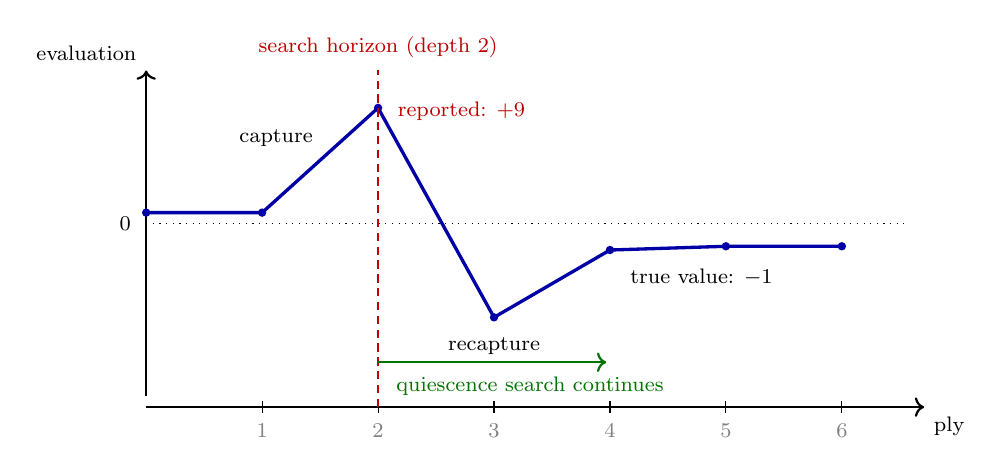
\begin{tikzpicture}[scale=0.95, transform shape, font=\small]
% evaluation axis (zero line kept separate from the ply axis)
\draw[->, thick] (0,-2.3) -- (0,2.05) node[above left, font=\footnotesize] {evaluation};
\draw[dotted] (0,0) -- (10.2,0);
\node[font=\footnotesize, anchor=east] at (-0.08,0) {$0$};

% ply axis, drawn below the curve so labels never touch it
\draw[->, thick] (0,-2.45) -- (10.4,-2.45) node[below right, font=\footnotesize] {ply};
\foreach \x/\lab in {1/1,2/2,3/3,4/4,5/5,6/6}{
  \draw (1.55*\x,-2.37) -- (1.55*\x,-2.53);
  \node[below, font=\footnotesize, gray] at (1.55*\x,-2.55) {\lab};
}

% evaluation trace: quiet, capture (+9), recapture (-1), quiet
\coordinate (p0) at (0,0.15);
\coordinate (p1) at (1.55,0.15);
\coordinate (p2) at (3.10,1.55);
\coordinate (p3) at (4.65,-1.25);
\coordinate (p4) at (6.20,-0.35);
\coordinate (p5) at (7.75,-0.30);
\coordinate (p6) at (9.30,-0.30);
\draw[very thick, blue!65!black] (p0) -- (p1) -- (p2) -- (p3) -- (p4) -- (p5) -- (p6);
\foreach \p in {p0,p1,p2,p3,p4,p5,p6}
  \fill[blue!65!black] (\p) circle (1.6pt);

% horizon at ply 2
\draw[red!75!black, thick, densely dashed] (3.10,-2.45) -- (3.10,2.05);
\node[red!75!black, font=\footnotesize, anchor=south] at (3.10,2.10)
  {search horizon (depth 2)};
\node[red!75!black, font=\footnotesize, anchor=west] at (3.24,1.50)
  {reported: $+9$};

% quiescence extension
\draw[->, green!45!black, thick] (3.10,-1.85) -- (6.15,-1.85);
\node[green!45!black, font=\footnotesize, anchor=north west] at (3.22,-1.92)
  {quiescence search continues};
\node[font=\footnotesize, anchor=west] at (6.35,-0.72) {true value: $-1$};

% annotations on the trace
\node[font=\footnotesize, anchor=east] at (2.35,1.15) {capture};
\node[font=\footnotesize, anchor=north] at (4.65,-1.40) {recapture};
\end{tikzpicture}
\caption{The horizon effect. The curve shows the static evaluation along a single
line of play in which a capture is answered by a recapture. A search limited to
two plies stops immediately after the capture and reports a decisive material
advantage that does not exist; one ply later the material is nearly balanced
again. Quiescence search resolves this by continuing beyond the nominal depth as
long as captures are available, and evaluating only once the position is quiet.}
\label{fig:horizon}
\end{figure}

In practice, quiescence search is commonly implemented using Alpha-Beta pruning
with a so-called \emph{stand-pat} evaluation~\cite{marsland1986review}, which
represents the static evaluation of the current position before any tactical
extensions are explored. If the stand-pat score already exceeds the current
bounds, the node can be pruned early.

Quiescence search significantly improves evaluation stability in tactical
positions and has become a standard component of classical chess engines. A
comprehensive discussion of the horizon effect and quiescence search can be
found in survey articles on game tree pruning~\cite{marsland1986review}.

\paragraph{Alpha-Beta Pruning}
Alpha-Beta pruning is an optimization technique that reduces the number of nodes
that need to be explored by Minimax or Negamax without affecting the correctness
of the final result. The technique was introduced by Knuth and Moore~\cite{knuth1975alphabeta}
and is a cornerstone of modern game tree search.

The algorithm maintains two bounds during search:
\begin{itemize}
    \item $\alpha$, the best score that the maximizing player can guarantee so
    far,
    \item $\beta$, the best score that the minimizing player can guarantee so
    far.
\end{itemize}

At the root of the search tree, $\alpha$ is initialized to $-\infty$ and $\beta$
to $+\infty$. As the search progresses, these bounds are updated based on the
values of explored child nodes. Whenever a node is encountered for which it can
be shown that its value cannot improve the current result, the corresponding
subtree is pruned and not searched further.

More concretely, during a maximizing step, the value of $\alpha$ is updated
whenever a better move is found. If $\alpha$ becomes greater than or equal to
$\beta$, further exploration of sibling nodes is unnecessary, as the minimizing
player would avoid reaching this position. An analogous argument applies during
minimizing steps.

\cref{fig:alphabeta} illustrates this on a minimal tree. The essential point is
that the pruned subtree is discarded without being looked at, and that this is
nevertheless safe: the discarded branch contains the highest leaf value of the
entire tree, but that value is never reachable, because the opponent decides at
that node and already holds a better alternative there. Pruning therefore removes
work, not information, which is what distinguishes Alpha-Beta from the heuristic
pruning discussed in \cref{subsec:null_move_pruning}.

\begin{figure}[ht]
\centering
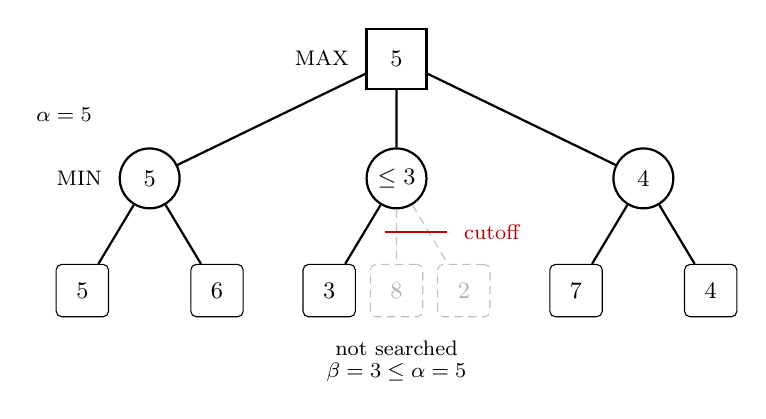
\begin{tikzpicture}[
  scale=0.95, transform shape,
  font=\small,
  maxn/.style={draw, thick, rectangle, minimum size=8mm, inner sep=1pt},
  minn/.style={draw, thick, circle, minimum size=8mm, inner sep=1pt},
  leaf/.style={draw, rectangle, rounded corners=2pt, minimum size=7mm, inner sep=2pt},
  gone/.style={draw=gray!50, densely dashed, rectangle, rounded corners=2pt,
               minimum size=7mm, inner sep=2pt, text=gray!60},
  edge/.style={-, thick},
  gedge/.style={-, gray!50, densely dashed}
]
% --- nodes -----------------------------------------------------------------
\node[maxn] (root) at (5,3.1) {$5$};
\node[left=1mm of root, font=\footnotesize] {MAX};

\node[minn] (a) at (1.7,1.5) {$5$};
\node[minn] (b) at (5,1.5)   {$\leq 3$};
\node[minn] (c) at (8.3,1.5) {$4$};
\node[left=1mm of a, font=\footnotesize] {MIN};

\node[leaf] (a1) at (0.8,0) {$5$};
\node[leaf] (a2) at (2.6,0) {$6$};
\node[leaf] (b1) at (4.1,0) {$3$};
\node[gone] (b2) at (5.0,0) {$8$};
\node[gone] (b3) at (5.9,0) {$2$};
\node[leaf] (c1) at (7.4,0) {$7$};
\node[leaf] (c2) at (9.2,0) {$4$};

% --- edges -----------------------------------------------------------------
\foreach \t in {a,b,c} \draw[edge] (root) -- (\t);
\foreach \t in {a1,a2} \draw[edge] (a) -- (\t);
\draw[edge] (b) -- (b1);
\foreach \t in {b2,b3} \draw[gedge] (b) -- (\t);
\foreach \t in {c1,c2} \draw[edge] (c) -- (\t);

% --- cut marker ------------------------------------------------------------
\draw[red!75!black, thick] (4.85,0.78) -- (5.68,0.78);
\node[red!75!black, font=\footnotesize, anchor=west] at (5.78,0.78) {cutoff};
\node[font=\footnotesize, align=center, anchor=north] at (5.0,-0.55)
  {not searched\\[-1pt]$\beta = 3 \leq \alpha = 5$};
\node[font=\footnotesize, align=left, anchor=east] at (1.05,2.35)
  {$\alpha = 5$};
\end{tikzpicture}
\caption{Alpha-Beta pruning on a minimal tree. The square root node maximizes,
the circular nodes minimize. The left subtree is searched first and yields $5$,
so the maximizing player is guaranteed at least $\alpha = 5$. In the middle
subtree the first leaf already returns $3$; since the minimizing player will
never choose more than $3$ there, this subtree cannot beat $5$ and its remaining
leaves are skipped, including the $8$, which is the largest value in the whole
tree. The result is identical to an exhaustive search, but two of the seven
leaves are never evaluated.}
\label{fig:alphabeta}
\end{figure}

\paragraph{Effectiveness and Influencing Factors}
In the worst case, Alpha-Beta pruning explores the same number of nodes as plain
Minimax. However, with optimal move ordering, the effective branching factor is
significantly reduced, allowing the search to reach roughly twice the depth of
unpruned Minimax for the same computational effort.

The effectiveness of Alpha-Beta pruning therefore depends strongly on the order
in which moves are explored. Techniques such as heuristic move ordering,
transposition tables, and iterative deepening are commonly employed to improve
this order and thereby increase pruning efficiency. These aspects are discussed
in more detail in \cref{sec:algorithm_implementation}.

\paragraph{Principal Variation Search}
Principal Variation Search (PVS) is a refinement of Alpha-Beta pruning that
exploits good move ordering even further~\cite{marsland1982parallel,
pearl1980scout}. The technique is based on the assumption that the first move
examined at a node is usually the best one. Only this first move is searched
with the full window $[\alpha, \beta]$. Every remaining move is first examined
with a so-called \emph{null window} (or zero window) $[\alpha, \alpha + 1]$,
which cannot return an exact score but can cheaply prove whether the move has
the potential to improve upon $\alpha$.

If the null-window search fails low, the move is confirmed to be inferior to
the current best move and no further work is required. If it fails high, the
assumption was wrong: the move may be better than the principal variation, and
the node must be \emph{re-searched} with the full window to obtain its exact
score. PVS therefore trades occasional re-searches for substantially cheaper
verification of the majority of moves. With strong move ordering, fail-highs
are rare and the technique reduces the overall search effort
considerably~\cite{reinefeld1983negascout}. Conversely, with poor move
ordering, frequent re-searches can negate the savings, which is why PVS is
typically combined with iterative deepening, transposition tables, and
heuristic move ordering.

For a comprehensive discussion of Alpha-Beta pruning and its variants in the
context of game-playing programs, see Marsland~\cite{marsland1986review}.

\subsection{Heuristic Evaluation}

Most positions encountered during search are non-terminal and therefore cannot be
assigned an exact game-theoretic value. Instead, they must be evaluated
heuristically. An evaluation function assigns a numerical score to a position,
indicating its desirability from the perspective of the side to move.

Classical evaluation functions combine material considerations with positional
features such as piece activity, king safety, and pawn structure. These features
are typically handcrafted and encode domain knowledge about the game of chess.
The design of the evaluation function has a significant impact on the playing
strength of the engine, particularly when search depth is limited.

Conceptually, the score returned by an evaluation function is expressed in a
common unit, most often \emph{centipawns}, where one pawn corresponds to a value
of $100$. Expressing heterogeneous factors, such as material imbalance and
positional advantages, on a single comparable scale allows them to be combined
into one number that the search can compare consistently across positions.

A refinement that is widely used in classical engines is the \emph{tapered}
evaluation. Since the relative importance of individual features changes over the
course of a game, for example when kings become active in the endgame, the
evaluation maintains two scores, one tuned for the midgame and one for the
endgame, and interpolates between them according to a game-phase measure derived
from the remaining material. The concrete evaluation used in this thesis follows
exactly this scheme and is described in detail in \cref{sec:evaluation_function}.

Finally, there is an inherent tension between the richness of the evaluation and
the depth of the search. A more detailed evaluation captures more chess knowledge
per node but is more expensive to compute, which reduces the number of nodes that
can be searched within a fixed time budget.

\subsection{Time-Constrained Search}

In practical settings, chess engines are required to operate under strict time
constraints. Rather than searching to a fixed depth, the engine must dynamically
adapt its search behavior to the available time budget.

\paragraph{Iterative Deepening}
Iterative deepening addresses this requirement by turning a single fixed-depth
search into a sequence of searches with increasing depth limit
$d = 1, 2, 3, \dots$, each starting again from the root~\cite{korf1985iterative}.
After every completed iteration the engine holds a fully valid best move for that
depth, so the search can be interrupted at essentially any point and still return
a well-founded decision. This \emph{anytime} property is precisely what makes the
technique well suited to time-controlled play, where the exact amount of
available time is not known in advance.

At first glance, repeatedly re-searching the shallow part of the tree appears
wasteful. In practice the overhead is small: because the number of nodes grows
exponentially with depth, the cost of the final iteration dominates the sum of
all previous ones, so re-searching depths $1$ to $d-1$ adds only a constant
factor to the cost of the depth-$d$ search. As discussed next, this overhead is
typically more than recovered through the improved move ordering that earlier
iterations provide.

\cref{fig:iterative_deepening} makes the two consequences of this exponential
growth visible at once. Because each iteration costs roughly three times its
predecessor, everything before the last one is nearly free, which is what makes
the repetition affordable. The same fact, however, means the engine faces an
all-or-nothing decision at every iteration boundary: the next iteration will
consume more time than the entire search so far, and if the clock runs out
half-way through it, that work is discarded entirely. Deciding whether to start
another iteration is therefore not a minor scheduling detail but the central
question of time management, and it is addressed in
\cref{sec:time_management}.

\begin{figure}[ht]
\centering
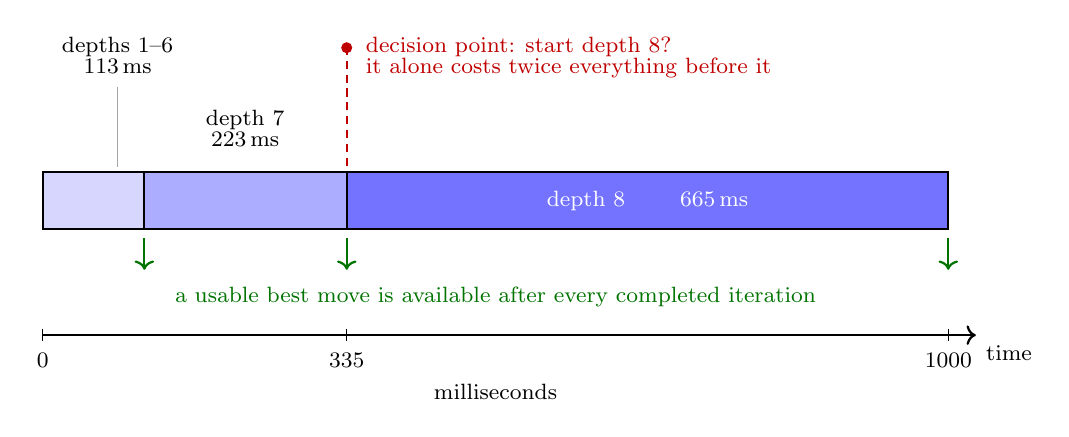
\begin{tikzpicture}[scale=1.0, font=\small]
% ---- the bar: widths proportional to measured cost per iteration ----------
\def\ybot{0}\def\ytop{0.72}
\fill[blue!16] (0,\ybot)    rectangle (1.29,\ytop);
\fill[blue!32] (1.29,\ybot) rectangle (3.86,\ytop);
\fill[blue!55] (3.86,\ybot) rectangle (11.5,\ytop);
\draw[thick] (0,\ybot) rectangle (11.5,\ytop);
\foreach \x in {1.29,3.86} \draw[thick] (\x,\ybot) -- (\x,\ytop);

% ---- segment labels ------------------------------------------------------
\node[font=\footnotesize, white] at (7.68,0.36) {depth 8 \qquad $665$\,ms};
\node[font=\footnotesize, align=center, anchor=south] at (2.57,0.92)
  {depth 7\\[-2pt]$223$\,ms};
\node[font=\footnotesize, align=center, anchor=south] at (0.95,1.85)
  {depths 1--6\\[-2pt]$113$\,ms};
\draw[gray!70] (0.95,1.80) -- (0.95,0.78);

% ---- time axis -----------------------------------------------------------
\draw[->, thick] (0,-1.35) -- (11.85,-1.35) node[below right, font=\footnotesize] {time};
\foreach \x/\lab in {0/0, 3.86/335, 11.5/1000}{
  \draw (\x,-1.27) -- (\x,-1.43);
  \node[below, font=\footnotesize] at (\x,-1.45) {\lab};
}
\node[below, font=\footnotesize] at (5.75,-1.85) {milliseconds};

% ---- soft stop decision --------------------------------------------------
\draw[red!75!black, thick, densely dashed] (3.86,\ytop+0.08) -- (3.86,2.30);
\fill[red!75!black] (3.86,2.30) circle (2pt);
\node[red!75!black, font=\footnotesize, anchor=south west, align=left]
  at (3.98,1.80) {decision point: start depth 8?\\[-2pt]
                  it alone costs twice everything before it};

% ---- anytime property ----------------------------------------------------
\foreach \x in {1.29,3.86,11.5}
  \draw[->, green!45!black, thick] (\x,-0.12) -- (\x,-0.52);
\node[green!45!black, font=\footnotesize, anchor=north] at (5.75,-0.62)
  {a usable best move is available after every completed iteration};
\end{tikzpicture}
\caption{Iterative deepening under a one-second budget, with the width of each
segment proportional to the time that iteration consumes. The proportions follow
from the effective branching factor of about $3$ measured for this engine in
\cref{subsec:eval_ttq}. The first six iterations together account for roughly a
tenth of the budget, so the repeated re-searching is cheap; the last iteration
alone accounts for two thirds. Every completed iteration leaves a valid best move
behind, which is what allows the search to be stopped at any point.}
\label{fig:iterative_deepening}
\end{figure}

\paragraph{Interaction with Pruning}
In addition to providing robustness under time constraints, iterative deepening
also improves the effectiveness of Alpha-Beta pruning. Information gathered in
earlier iterations, such as good move orderings, can be reused in deeper searches,
leading to a significant reduction in the number of explored nodes.

\paragraph{Search Tree Reuse Across Searches}
The same principle extends beyond a single search invocation. After the engine
has played a move and the opponent has responded, the new search root lies
within the tree that was explored during the previous search. If the results of
that search are retained, for example in a transposition table, the engine can
\emph{resume} the old search tree: previously computed scores yield immediate
cutoffs, and previously identified best moves improve the move ordering from the
very first iteration. Conceptually, the engine no longer starts each search from
scratch but continues the computation it has already begun in earlier moves of
the game.

The interaction between heuristic evaluation, Alpha-Beta pruning, and
time-constrained iterative deepening forms the foundation of modern chess
engines and is a central aspect of this work.

\cleardoublepage
\section{Algorithm \& Implementation}
\label{sec:algorithm_implementation}

This section describes the algorithms used by the engine and how they were
implemented. It first introduces the overall engine architecture and the
baseline search, consisting of Negamax with Alpha-Beta pruning, iterative
deepening, quiescence search, transposition tables, and heuristic move ordering.
Building on this baseline, the two main algorithmic improvements of this thesis
are presented: Principal Variation Search and the reuse of search trees from
previous searches. The section concludes with the time management scheme and
the static evaluation function.

\section{Engine Architecture}
\label{sec:architecture}

This section describes the overall architecture of the implemented chess engine.
The focus lies on the structural design decisions and the interaction between the
core components. Rather than optimizing for maximum playing strength, the
architecture is deliberately kept modular and transparent in order to facilitate
experimentation and detailed analysis of search algorithms and time management
strategies.

\subsection{Overall Design}

The engine follows a layered architecture that separates game representation,
move generation, search, evaluation, and search control. Each component has a
clearly defined responsibility and communicates with other modules through
narrow and explicit interfaces.

\cref{fig:architecture} provides a high-level overview of the engine structure
and the interaction between the individual modules.

\begin{figure}[ht]
\centering
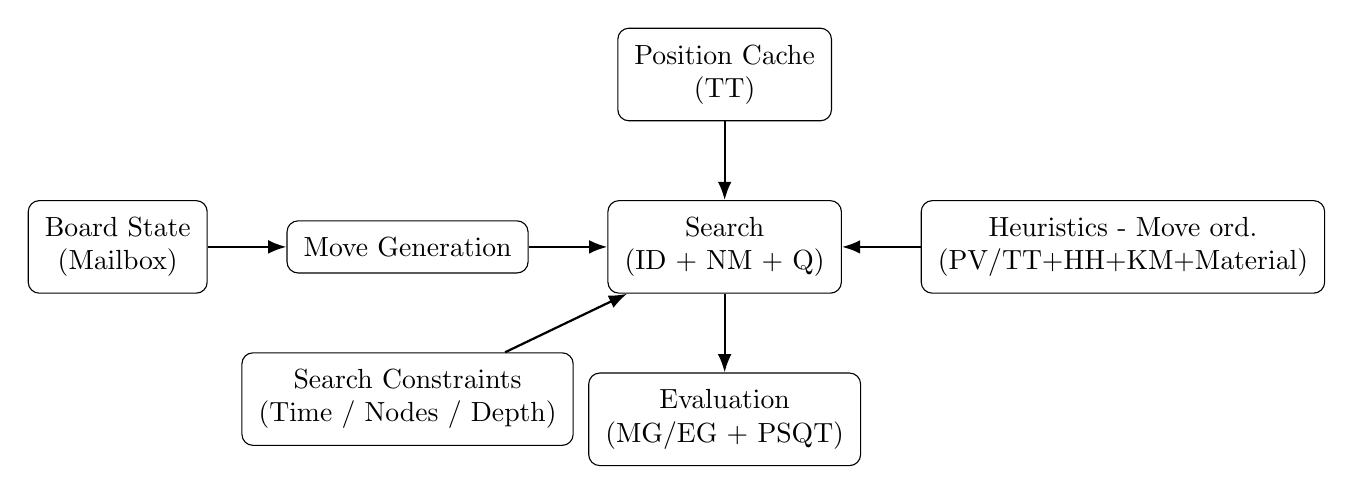
\begin{tikzpicture}[
  box/.style={draw, rounded corners, inner sep=6pt, align=center},
  arr/.style={-Latex, thick}
]
\node[box] (board) {Board State\\(Mailbox)};
\node[box, right=1cm of board] (movegen) {Move Generation};
\node[box, right=1cm of movegen] (search) {Search\\(ID + NM + Q)};
\node[box, below=1cm of search] (eval) {Evaluation\\(MG/EG + PSQT)};
\node[box, above=1cm of search] (tt) {Position Cache\\(TT)};
\node[box, below=1cm of movegen] (time) {Search Constraints\\(Time / Nodes / Depth)};
\node[box, right=1cm of search] (heuristics) {Heuristics - Move ord.\\(PV/TT+HH+KM+Material)};

\draw[arr] (board) -- (movegen);
\draw[arr] (movegen) -- (search);
\draw[arr] (search) -- (eval);
\draw[arr] (tt) -- (search);
\draw[arr] (time) -- (search);
\draw[arr] (heuristics) -- (search);
\end{tikzpicture}
\caption{High-level architecture of the implemented chess engine.}
\label{fig:architecture}
\end{figure}

At a conceptual level, the engine consists of the representation of the game
state, the generation and application of moves, the search procedure, the static
evaluation, and a unified constraint mechanism that controls search termination.
This separation ensures that individual components can be modified or replaced
without affecting the rest of the system, which is particularly important for
experimental analysis.

\subsection{Game State and Move Handling}

\paragraph{Board Representation}
The board is represented using a classical mailbox model consisting of 64
squares. Each square explicitly stores the occupying piece or indicates that the
square is empty. In addition to the piece placement, the board state contains
information about the side to move, castling rights, king squares and en-passant availability.

Modern state-of-the-art engines typically rely on bitboard-based representations
for efficient move generation and evaluation. However, mailbox representations
remain a common choice in educational and experimental engines due to their
simplicity and transparency~\cite{cpw_bitboards}. Given the focus of this work on
algorithmic behavior rather than raw performance, the mailbox model provides a
clear and easily analyzable foundation.

\paragraph{Move Representation}
Moves are represented as explicit objects containing all information required to
apply and undo them. This includes the source and destination squares, the moving
piece, captured pieces, promotion information, and special move flags for
castling, promotion and en-passant captures.

This design enables a fully reversible make--unmake mechanism, which is essential
for recursive search algorithms. By storing all relevant information directly in
the move object, the engine avoids recomputation when restoring previous board
states, thereby simplifying the search implementation and reducing potential
sources of errors.

\paragraph{Move Generation}
Move generation follows a direct and exhaustive approach. For each piece on the
board, all potential target squares are examined according to the rules of
chess. No precomputed attack tables or bitboard-based optimizations are used.

Illegal moves, such as those that leave the king in check, are filtered during
move execution rather than during generation. This design keeps the move
generator independent of check detection logic and makes its behavior easier to
reason about. Although this approach is less optimized than state-of-the-art
alternatives, it provides a robust and well-understood baseline for search
experimentation.

\subsection{Position Hashing and Transposition Tables}

\paragraph{Zobrist Hashing}
To uniquely identify board positions, the engine employs Zobrist hashing. Each
combination of square and piece type is associated with a random 64-bit value,
and the hash of a position is computed by XOR-combining the values corresponding
to the pieces currently on the board. Additional state information, such as the
side to move, castling rights, and en-passant availability, is also incorporated
into the hash.

Zobrist hashing is commonly used in game tree search because it allows board
positions to be mapped efficiently to fixed-size keys. While the technique
supports incremental updates during make--unmake operations, the implementation
used in this engine recomputes the hash from the board state directly. The technique itself was originally introduced by Zobrist~\cite{zobrist1970hashing} and has since become a standard component of modern chess engines.

\paragraph{Transposition Table Usage}
The computed hash values are used as keys in a transposition table, which stores
previously evaluated positions. Each entry contains the evaluation score, the
search depth at which the position was evaluated, a bound type (exact, lower
bound, or upper bound), and the best move found.

The transposition table serves two closely related purposes. First, it reduces
search redundancy by reusing results for positions that can be reached via
different move orders, which is common in chess. Without such a mechanism,
identical positions would be evaluated repeatedly, leading to a significant
increase in search effort. Second, transposition table entries improve move
ordering by prioritizing moves that proved effective in previous searches. A
simple aging mechanism ensures that outdated entries are gradually replaced,
preventing the table from being dominated by stale information. For practical
implementations and further discussion, see for example Warnock~\cite{warnock1988search}.

\subsection{Search Control and Integration}

\paragraph{Unified Search Constraints}
All termination conditions for a search invocation are encapsulated in a single
constraint structure. This includes depth limits, node limits, time budgets, and
special modes such as infinite search or pondering.

Encapsulating all stopping criteria in a unified constraint object avoids
scattered stop checks throughout the search code and ensures consistent behavior
across different search modes. This design is particularly important for
experimental analysis, as it guarantees that differences in search behavior are
caused by the chosen constraints rather than by implementation artifacts.

\paragraph{Engine Integration}
The engine core is coordinated by a game management component that maintains the
current position, applies and reverts moves, and invokes the search procedure.
This component acts as a bridge between the external UCI interface and the
internal search and evaluation modules, ensuring a clean separation between
protocol handling and algorithmic logic.

\subsection{Design Rationale}

The architectural decisions made in this engine deliberately prioritize clarity,
correctness, and experimental flexibility over maximum playing strength. Many
state-of-the-art engines employ highly optimized data structures and aggressive
micro-optimizations, which can obscure the underlying algorithmic behavior.

By choosing a modular and explicit design, this engine allows the effects of
search algorithms, heuristics, and time management strategies to be studied in
isolation. This aligns with the primary goal of this work, which is to analyze
the behavior of iterative deepening search under time constraints rather than to
compete directly with top-performing chess engines.

\subsection{Search Algorithms}
\label{sec:search}

The underlying algorithms (Negamax, Alpha-Beta pruning, and quiescence search)
were introduced in \cref{sec:preliminaries}. This subsection turns to their
concrete realization in code and to how the individual mechanisms interact in
practice. Particular attention is paid to the two refinements of
this thesis: the move loop is organized as a Principal Variation Search
(\cref{subsec:pvs_implementation}), and previous search trees are resumed
through the persistent transposition table (\cref{subsec:tree_reuse}).

\subsubsection{Search Entry Point and Modes}

The main entry point is \texttt{ChessBot::think()}, which receives the board
together with a \texttt{SearchConstraints} object. The constraints are copied
intentionally and stored inside the engine instance for the duration of the
search. Before searching, the engine
initializes a clean state via \texttt{reset\_search\_state()}, which resets node
counters, selective depth tracking, stop state, and heuristic tables (killer and
history), and also advances the transposition table generation via
\texttt{tt.new\_search()}.

Depending on \texttt{config.mode\_}, the engine selects one of the following
execution strategies:
\begin{itemize}
    \item \textbf{FixedDepth:} the time budget is explicitly disabled
    (\texttt{budget\_ = \{\}}) to prevent time-based termination inside
    \texttt{hard\_stop()}. The engine performs a single root search with the
    requested depth and returns the result.
    \item \textbf{NodeLimit / Infinite:} time-based termination is disabled and
    the engine runs iterative deepening until an external stop condition
    (or the node limit) is hit.
    \item \textbf{Normal / FixedTime (time-managed):} the \texttt{TimeManager}
    initializes a soft and hard deadline from the constraints, and iterative
    deepening runs under these deadlines.
\end{itemize}

This structure keeps the actual search logic independent of UCI parsing and
ensures that all termination behavior is expressed through the constraint object
and the common stop checks.

\subsubsection{Termination and Safety Checks}

All immediate termination decisions are centralized in
\texttt{ChessBot::hard\_stop()}, which is called frequently inside the search
(including quiescence) and combines an external stop flag, the hard time
deadline, and an optional node budget. The exact semantics of these criteria,
and the distinction between the hard deadline and the \emph{soft} deadline that
is only consulted between completed iterations of iterative deepening, are
described in \cref{sec:time_management}.

The stop flag and the node budget are checked at every node, the clock only every
1024 nodes. Reading a monotonic clock costs considerably more than the comparison
it guards, and at the node rates the engine reaches, the resulting imprecision
stays below a millisecond.

As an additional robustness measure, the engine verifies the final move before
returning it. If the selected move is not legal (checked via
\texttt{is\_legal\_move()}), the engine falls back to a legal move
obtained from \texttt{get\_legal\_fallback\_move()}.

\subsubsection{Iterative Deepening Loop}

Time-managed searches run in \texttt{ChessBot::iterative\_deepening(Board\&)}.
The engine starts with a legal fallback move and then performs repeated searches
with increasing depth $d = 1,2,3,\dots$.

For each iteration, a local copy of the current best move is passed into
\texttt{root\_search()}. If the search completes successfully, the resulting move
becomes the new best move and is reported via the UCI \texttt{info} output
(\texttt{print\_info}). If an iteration is aborted (e.g., due to a hard stop),
the loop terminates and the engine returns the best move from the last completed
iteration.

Hard stops are enforced immediately inside the search, while soft stops only
take effect at iteration boundaries (cf. \cref{sec:time_management}).

\subsubsection{Root Search and Core Negamax}

The helper \texttt{root\_search(Board\&, depth, Move\&)} is a thin wrapper that
invokes Negamax with the initial window $[-\infty, +\infty]$ and ply $0$.
The best move is returned through the referenced move parameter, which avoids
additional return-value plumbing and keeps the recursive signature compact.

The core search routine \texttt{ChessBot::negamax(...)} implements a standard
depth-limited Negamax with Alpha-Beta bounds:
\begin{itemize}
    \item If \texttt{depth <= 0}, the search transitions into quiescence search.
    \item At every node, \texttt{hard\_stop()} may terminate the search early.
    \item The routine maintains and updates $\alpha$ during move exploration; a
    cutoff occurs when $\alpha \ge \beta$.
\end{itemize}

To support correct transposition table storage, the implementation stores the
original alpha value (\texttt{ORIGINAL\_ALPHA}) and uses it later to classify the
result as \texttt{EXACT}, \texttt{LOWER\_BOUND}, or \texttt{UPPER\_BOUND}.

\paragraph{Legal Move Handling}
Moves are generated as pseudo-legal moves and filtered by attempting to apply
them with \texttt{board.make\_move(move)}. If \texttt{make\_move} fails (e.g.,
because the move leaves the king in check), the move is discarded. This design
keeps move generation simpler and delegates legality to the make--unmake layer,
which also guarantees that the search only recurses into legal positions.

\paragraph{Terminal Positions}
If no legal move exists, the implementation distinguishes:
\begin{itemize}
    \item \textbf{checkmate:} if the side to move is in check, return a mate score
    of the form $-(MATE - ply)$,
    \item \textbf{stalemate:} otherwise return $0$.
\end{itemize}
Using the current ply in the mate score ensures that faster mates are preferred
and slower mates are avoided.

\subsubsection{Principal Variation Search}
\label{subsec:pvs_implementation}

The move loop inside \texttt{negamax} implements the Principal Variation Search
scheme introduced in \cref{sec:preliminaries}. Instead of searching every move
with the full window $[\alpha, \beta]$, the engine searches only the leading
moves with the full window and verifies all remaining moves with a null-window
search $[\alpha, \alpha + 1]$ (realized as $[-\alpha - 1, -\alpha]$ in the
Negamax formulation). Only if the null-window search indicates that a move can
beat $\alpha$ without already exceeding $\beta$ is the move re-searched with
the full window to obtain its exact score.

The behavior is controlled by two tunable parameters bundled in a
\texttt{PvsConfig} structure:
\begin{itemize}
    \item \texttt{min\_depth} (default $2$): below this remaining depth the
    scout search is skipped entirely and all moves are searched with the full
    window. At shallow nodes the subtrees are so small that the potential
    re-search overhead would outweigh the savings of the null-window search.
    \item \texttt{scout\_after\_move} (default $1$): the first $N$ legal
    moves of a node are always searched with the full window. Move ordering is
    least reliable for the very first moves, so the engine only switches to the
    cheap null-window scout once the presumed principal variation has been
    established.
\end{itemize}

Both parameters are exposed as UCI options (\texttt{PvsMinDepth} and
\texttt{PvsScoutAfterMove}), which allows the scouting behavior to be tuned and
evaluated experimentally without recompiling the engine. The overall structure
of the move loop is summarized in \cref{algo:pvs}.

\begin{algorithm}[ht]
\DontPrintSemicolon
\KwIn{Position $P$, depth $d$, bounds $\alpha, \beta$, legal move counter $n$}
\KwOut{Score of the searched move}

\uIf{$n < \texttt{scout\_after\_move}$ \textbf{or} $d < \texttt{min\_depth}$}{
    $score \gets -\textsc{Negamax}(P, d-1, -\beta, -\alpha)$\tcp*{full window}
}
\Else{
    $score \gets -\textsc{Negamax}(P, d-1, -\alpha - 1, -\alpha)$\tcp*{null-window scout}
    \If{$\alpha < score < \beta$}{
        $score \gets -\textsc{Negamax}(P, d-1, -\beta, -\alpha)$\tcp*{re-search}
    }
}
\Return $score$\;
\caption{Principal Variation Search inside the Negamax move loop.}
\label{algo:pvs}
\end{algorithm}

A subtle but important implementation detail is the interaction with aborted
searches: if a null-window scout is aborted by a hard stop, its score is not
trusted and no re-search is triggered; instead, the abort is propagated upward
so that the iterative deepening loop can discard the incomplete iteration.

\subsubsection{Quiescence Search}
\label{subsec:quiescence_impl}

Quiescence search is implemented in \texttt{ChessBot::quiescence(...)} and is
entered whenever the regular search reaches depth $0$. The function evaluates
the current position via \texttt{eval::evaluate(board)} and then selectively
extends the search by exploring only tactical moves (captures and en-passant).
Non-capturing moves are skipped explicitly. The captures are filtered out of the
generated list before the list is ordered, so the ordering only has to run over
the handful of moves that are actually searched instead of over all of them.

The implementation uses the standard \emph{stand-pat} scheme:
\begin{itemize}
    \item if the static score already exceeds $\beta$, the node fails high,
    \item otherwise $\alpha$ is updated using the static score and improved
    through capture exploration.
\end{itemize}

As with the main search, \texttt{hard\_stop()} is checked inside quiescence to
enforce hard termination constraints consistently.

\subsubsection{Null-Move Pruning}
\label{subsec:null_move_pruning}

In addition to the exact Alpha-Beta framework, the engine applies null-move
pruning as a forward-pruning enhancement of the baseline search. The underlying
observation is that in most positions having the right to move is an advantage:
if a side is allowed to skip its turn (a \emph{null move}) and the resulting
position, searched to a reduced depth, is still good enough to produce a beta
cutoff, then the position is almost certainly too strong for the opponent and the
whole subtree can be pruned without a full-depth search. The technique goes back
to Beal~\cite{beal1989nullmove} and is a standard component of classical engines.

\cref{fig:nullmove} contrasts the two searches involved. The decisive property is
that the reduced search answers a deliberately easier question than the one the
node actually poses. It grants the opponent a free move and still finds the
position too good, which is strong evidence that the node would also survive a
proper search. Unlike Alpha-Beta this is evidence rather than proof, and the
figure also indicates where it breaks down: in zugzwang positions, having to move
is a disadvantage, so passing improves rather than worsens the position and the
inference is invalid. This is the reason for the guard conditions listed below.

\begin{figure}[ht]
\centering
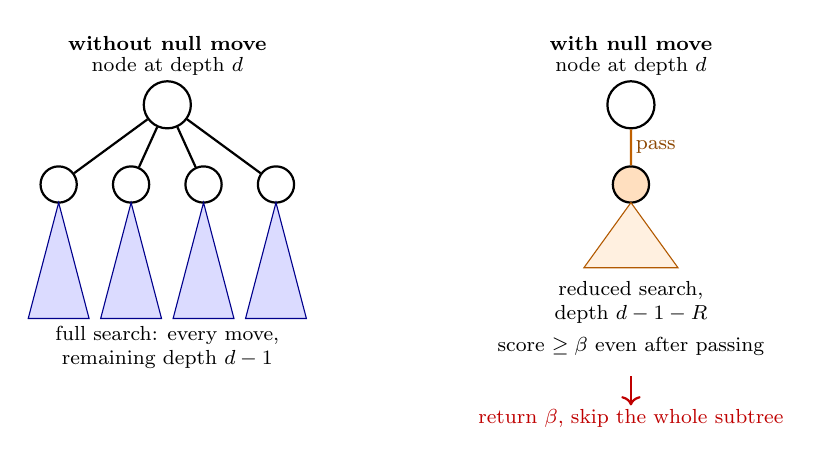
\begin{tikzpicture}[
  scale=0.92, transform shape, font=\small,
  nd/.style={draw, thick, circle, minimum size=6.5mm, inner sep=0pt},
  lbl/.style={font=\footnotesize, inner sep=1.5pt}
]
% ---------------- left: what the node would cost --------------------------
\begin{scope}
  \node[nd] (r) at (2,2.6) {};
  \node[lbl, anchor=south] at (2,2.95) {node at depth $d$};
  \foreach \i/\x in {1/0.5,2/1.5,3/2.5,4/3.5}{
    \node[nd, minimum size=5mm] (m\i) at (\x,1.5) {};
    \draw[thick] (r) -- (m\i);
  }
  \foreach \i/\x in {1/0.5,2/1.5,3/2.5,4/3.5}
    \draw[fill=blue!14, draw=blue!55!black] (\x,1.25) -- (\x-0.42,-0.35) -- (\x+0.42,-0.35) -- cycle;
  \node[lbl, align=center] at (2,-0.75) {full search: every move,\\remaining depth $d-1$};
  \node[font=\footnotesize\bfseries] at (2,3.45) {without null move};
\end{scope}
% ---------------- right: the null-move probe ------------------------------
\begin{scope}[xshift=6.4cm]
  \node[nd] (R) at (2,2.6) {};
  \node[lbl, anchor=south] at (2,2.95) {node at depth $d$};
  \node[nd, minimum size=5mm, fill=orange!25] (P) at (2,1.5) {};
  \draw[thick, orange!75!black] (R) -- node[lbl, right, text=orange!55!black] {pass} (P);
  \draw[fill=orange!12, draw=orange!70!black] (2,1.25) -- (1.35,0.35) -- (2.65,0.35) -- cycle;
  \node[lbl, align=center, anchor=north] at (2,0.22) {reduced search,\\depth $d-1-R$};
  \node[lbl, align=center, anchor=north] at (2,-0.55)
    {score $\geq \beta$ even after passing};
  \draw[->, red!75!black, thick] (2,-1.15) -- (2,-1.55);
  \node[lbl, align=center, anchor=north, text=red!75!black] at (2,-1.55)
    {return $\beta$, skip the whole subtree};
  \node[font=\footnotesize\bfseries] at (2,3.45) {with null move};
\end{scope}
\end{tikzpicture}
\caption{Null-move pruning. Instead of searching every move at full depth (left),
the engine first lets the side to move pass and searches the resulting position
to a reduced depth (right). If the position is still good enough to exceed
$\beta$ despite this handicap, the node is assumed to be beyond the opponent's
reach and the subtree is skipped. The saving is large because the probe is both
shallower and single-branched, but the inference is heuristic: it fails in
zugzwang, where passing would be an improvement rather than a concession.}
\label{fig:nullmove}
\end{figure}

The pruning is performed inside \texttt{negamax}, after the transposition table
probe but before the moves are generated and ordered. The engine plays a null
move via \texttt{board.make\_null\_move()}, searches the resulting position to a
reduced depth $d-1-R$ with a null window around $\beta$ (realized as
$[-\beta, -\beta+1]$ in the Negamax formulation), and restores the position with
\texttt{board.pop\_null\_move()}. If the returned score satisfies
$-\text{score} \ge \beta$, the node fails high and $\beta$ is returned directly.
The number of such cutoffs is tracked in the \texttt{null\_cutoffs} counter for
the experimental instrumentation.

Because null-move pruning is a heuristic rather than an exact technique, it is
guarded by several conditions. The reduced search is only attempted when all of
the following hold:
\begin{itemize}
    \item pruning is enabled and this node was not already reached through a null
    move (\texttt{can\_null}); two consecutive passes are never searched, as they
    correspond to no meaningful line of play,
    \item the node is not the root ($ply > 0$), since the root must always return
    a real best move,
    \item the remaining depth is at least \texttt{min\_depth}; below this the
    reduced search would be too shallow to justify the risk,
    \item $\beta$ is not already a mate score
    ($|\beta| < \texttt{kMate} - \texttt{kMateWindow}$), because a fabricated
    move would distort mate distances,
    \item the side to move is not in check, since passing while in check would
    leave the king en prise,
    \item the side to move still has non-pawn material
    (\texttt{has\_non\_pawn\_material}); in pawn-only endgames zugzwang makes
    passing frequently favourable, which would invalidate the pruning assumption.
\end{itemize}

As in the rest of the search, an aborted reduced search is not trusted: if the
null-move search is terminated by a hard stop, the abort is propagated upward and
no cutoff is derived from the incomplete result. The behaviour is controlled by a
\texttt{NullMoveConfig} structure exposing whether the technique is enabled, the
minimum remaining depth (\texttt{min\_depth}, default $3$), and the depth
reduction (\texttt{reduction}, default $2$). All three are exposed as the UCI
options \texttt{NullMove}, \texttt{NullMoveMinDepth}, and
\texttt{NullMoveReduction}, so the pruning can be toggled and tuned without
recompiling.

\subsubsection{Transposition Table Integration}

The motivation for the table is that the game tree is not, strictly speaking, a
tree. Different sequences of moves frequently lead to the identical position, so
the same node appears many times over at the same depth. A plain recursive search
has no way of noticing this and re-solves each occurrence from scratch, which is
pure duplicated work. \cref{fig:transposition} shows the effect in its smallest
form. Storing results under a hash of the position turns the traversal from a
tree into a directed acyclic graph and lets the second occurrence be answered
from memory. Since the number of such collisions grows with depth, this is one of
the few techniques whose benefit increases rather than decreases as the search
gets deeper, which is also why the same table can be carried across moves
(\cref{subsec:tree_reuse}).

\begin{figure}[ht]
\centering
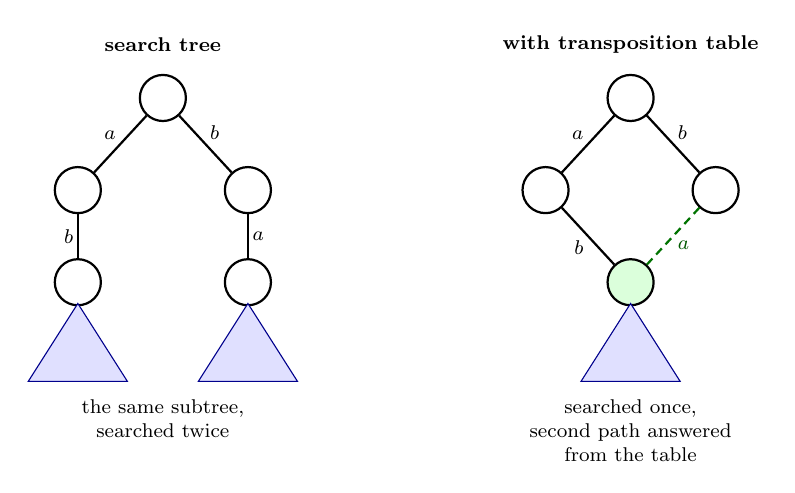
\begin{tikzpicture}[
  scale=0.9, transform shape, font=\small,
  nd/.style={draw, thick, circle, minimum size=6.5mm, inner sep=0pt},
  lbl/.style={font=\footnotesize, inner sep=1.5pt}
]
% ---------------- left: plain tree ----------------
\begin{scope}
  \node[nd] (r) at (2,3) {};
  \node[nd] (x1) at (0.8,1.7) {};
  \node[nd] (x2) at (3.2,1.7) {};
  \node[nd] (y1) at (0.8,0.4) {};
  \node[nd] (y2) at (3.2,0.4) {};
  \draw[thick] (r) -- node[lbl,above left] {$a$} (x1);
  \draw[thick] (r) -- node[lbl,above right] {$b$} (x2);
  \draw[thick] (x1) -- node[lbl,left] {$b$} (y1);
  \draw[thick] (x2) -- node[lbl,right] {$a$} (y2);
  \draw[fill=blue!12, draw=blue!55!black] (0.8,0.1) -- (0.1,-1.0) -- (1.5,-1.0) -- cycle;
  \draw[fill=blue!12, draw=blue!55!black] (3.2,0.1) -- (2.5,-1.0) -- (3.9,-1.0) -- cycle;
  \node[lbl, align=center, anchor=north] at (2,-1.20) {the same subtree,\\searched twice};
  \node[font=\footnotesize\bfseries] at (2,3.75) {search tree};
\end{scope}
% ---------------- right: DAG ----------------
\begin{scope}[xshift=6.6cm]
  \node[nd] (R) at (2,3) {};
  \node[nd] (X1) at (0.8,1.7) {};
  \node[nd] (X2) at (3.2,1.7) {};
  \node[nd, fill=green!14] (Y) at (2,0.4) {};
  \draw[thick] (R) -- node[lbl,above left] {$a$} (X1);
  \draw[thick] (R) -- node[lbl,above right] {$b$} (X2);
  \draw[thick] (X1) -- node[lbl,below left] {$b$} (Y);
  \draw[thick, densely dashed, green!45!black] (X2) --
        node[lbl,below right, text=green!35!black] {$a$} (Y);
  \draw[fill=blue!12, draw=blue!55!black] (2,0.1) -- (1.3,-1.0) -- (2.7,-1.0) -- cycle;
  \node[lbl, align=center, anchor=north] at (2,-1.20) {searched once,\\second path answered\\from the table};
  \node[font=\footnotesize\bfseries] at (2,3.75) {with transposition table};
\end{scope}
\end{tikzpicture}
\caption{Transpositions. Playing move $a$ and then $b$ leads to exactly the same
position as playing $b$ and then $a$, so a plain recursive search explores the
identical subtree twice (left). A transposition table stores the result of the
first visit under a hash of the position, so the second path finds it already
solved and returns immediately (right). Real search trees contain vastly more
such convergences than this minimal example suggests.}
\label{fig:transposition}
\end{figure}

The search consults the transposition table early in \texttt{negamax} via
\texttt{tt.probe(key, depth, alpha, beta, ply, ...)}. A successful probe may:
\begin{itemize}
    \item return an \texttt{EXACT} score,
    \item produce a safe cutoff using stored \texttt{LOWER\_BOUND} or
    \texttt{UPPER\_BOUND} information.
\end{itemize}

In addition, the table provides a stored best move (\texttt{tt\_move}) which is
used for move ordering. Since transposition table entries may be stale or collide,
the implementation verifies the move's legality before using it; illegal TT moves
are discarded.

After searching a node, the result is stored via \texttt{tt.store(...)} together
with the depth, bound type, and the best move found at that node. Mate scores are
encoded in a TT-safe form using the ply (via \texttt{to\_tt\_score} /
\texttt{from\_tt\_score}) so that mate distances remain consistent across
different search depths.

\subsubsection{Search Tree Reuse Across Searches}
\label{subsec:tree_reuse}

The transposition table is not only used within a single search invocation but
also serves as the engine's mechanism for resuming previous search trees. The
table is a member of the engine instance and is deliberately \emph{not} cleared
between searches. When a new search starts, \texttt{reset\_search\_state()}
only calls \texttt{tt.new\_search()}, which advances an internal generation
counter; all stored entries remain accessible. A full \texttt{tt.clear()} is
performed only when the UCI command \texttt{ucinewgame} signals that an
entirely new game begins.

This design directly implements the idea of continuing an earlier computation.
After the engine has played a move and the opponent has answered, the new root
position lies inside the tree that was explored during the previous search.
Probing the persistent table therefore immediately recovers large parts of the
earlier work:
\begin{itemize}
    \item \textbf{Score reuse:} entries stored with sufficient depth yield
    exact scores or safe bound cutoffs without re-searching the corresponding
    subtrees.
    \item \textbf{Move ordering reuse:} stored best moves from the previous
    search guide the move ordering of the new search from the very first
    iteration, which is exactly the situation in which Principal Variation
    Search and Alpha-Beta pruning are most effective.
\end{itemize}

The generation counter implements a soft aging scheme rather than hard
invalidation. The replacement policy prefers overwriting entries from older
generations and entries with lower depth, so stale information gradually
disappears as the game progresses while still being available as long as it is
not displaced. In combination with iterative deepening, this means consecutive
searches behave less like independent computations and more like one continuous
search that is deepened and re-rooted as the game advances.

Keeping the table alive across searches has one consequence that a table cleared
per search does not have: a stored move outlives the position it was generated
for. Since the table is indexed by a truncated key, two different positions can
map to the same entry, and the move handed back then describes pieces that are no
longer where it expects them. Such a move is not merely bad, it is not playable at
all, and applying it would corrupt the board rather than just cost search time.
Every move taken from the table is therefore validated against the current
position before it is used as an answer: it has to be one the move generator
produces here, and it must not leave the own king in check. Moves that come
straight from the generator need no such check, they are pseudo-legal by
construction, so the validation is confined to the few places where a move of
foreign origin enters the search.

\subsubsection{Move Ordering and Heuristics}
\label{subsec:move_ordering}

Move ordering is implemented in \texttt{search::heuristics::order\_moves}.
The ordering score combines several standard heuristics, all of which are
surveyed by Marsland~\cite{marsland1986review}:
\begin{itemize}
    \item \textbf{TT/PV move first:} if a transposition table move exists, it
    receives a large bonus and is sorted to the front.
    \item \textbf{Captures before quiet moves:} captures are prioritized using a
    MVV-LVA-inspired score (most valuable victim / least valuable attacker),
    with a special case for en-passant.
    \item \textbf{Killer moves:} for each ply, the engine tracks up to two quiet
    moves that previously caused beta cutoffs and boosts them in ordering.
    \item \textbf{History heuristic}~\cite{schaeffer1989history}\textbf{:} a 3D
    table indexed by side, from-square, and to-square accumulates bonuses (scaled
    by depth squared) for quiet moves that caused cutoffs, and the accumulated
    score is added during ordering.
\end{itemize}

Killer and history updates are performed only on beta cutoffs and only for quiet
moves. This avoids polluting these tables with captures and ensures that the
heuristics reflect moves that are generally useful for pruning rather than
tactical one-offs.

\subsubsection{Debugging and Instrumentation}

The search provides UCI-compliant reporting via \texttt{print\_info}, including
depth, selective depth, time, nodes, NPS, and either centipawn score or mate
distance (converted from the internal mate representation). Additionally, a
configurable debug facility can emit search health statistics, transposition
table statistics, root move ordering, and principal variation output. This
instrumentation supports the experimental goal of this thesis by making search
behavior observable and reproducible.

\section{Time Management and Constraints}
\label{sec:time_management}

In practical chess engines, search is not only limited by depth but often by a
set of external constraints such as time, node budgets, or explicit stop
signals. In this engine, all stopping conditions for a single search invocation
are bundled in an immutable constraint object, which is initialized once before
the search starts and treated as read-only during the search.

A key design goal is that the search code itself does not depend on UCI parsing
details. Instead, the UCI layer produces a fully specified \texttt{SearchConstraints}
instance, and the search only consults this object (and a stop flag) to decide
when to terminate.

\subsection{Unified Constraint Model}

The engine uses a dedicated \texttt{SearchConstraints} structure to describe how
a search is controlled and when it should terminate. This structure unifies all
search modes under a single interface and avoids scattered termination logic
across the search code.

A constraint instance contains:
\begin{itemize}
    \item a \textbf{search mode} determining which criteria are active,
    \item an optional \textbf{fixed move time} (\texttt{movetime\_ms\_}),
    \item an optional \textbf{fixed depth} (\texttt{depth\_}),
    \item an optional \textbf{node limit} (\texttt{nodes\_}),
    \item and a \textbf{time budget} object (\texttt{budget\_}) used for time-managed searches.
\end{itemize}

To simplify checks in the search, convenience predicates such as
\texttt{has\_fixed\_depth()}, \texttt{has\_node\_limit()}, and \texttt{has\_movetime()}
are provided.

\subsection{Search Modes}

The active search behavior is selected via \texttt{SearchType}. The engine
supports the following modes:
\begin{itemize}
    \item \textbf{Normal:} Tournament-style time management with iterative
    deepening (default UCI behavior). Time allocation is derived from the clock
    settings and stored in \texttt{budget\_}.
    \item \textbf{FixedTime:} Search for a fixed amount of time specified by
    \texttt{movetime\_ms\_} (UCI \texttt{go movetime}).
    \item \textbf{FixedDepth:} Search to a fixed depth only, determined by
    \texttt{depth\_}, without relying on time control.
    \item \textbf{NodeLimit:} Search until a fixed number of nodes specified by
    \texttt{nodes\_} has been explored.
    \item \textbf{Infinite:} Search indefinitely until an external stop command
    is received (UCI \texttt{go infinite}).
    \item \textbf{Ponder:} Search during the opponent’s time. The engine
    continues searching until it is either stopped or the predicted opponent
    move is played, at which point the search can be continued or restarted.
\end{itemize}

This mode-based design enables a clean separation between the UCI interface
(which interprets the \texttt{go} command) and the search itself (which only
consults the active constraints).

\subsection{Time Budgets: Structure and Arming}

Time-based searches (Normal / FixedTime) rely on \texttt{TimeControl} stored in
\texttt{SearchConstraints::budget\_}. The budget distinguishes a \emph{soft} and a
\emph{hard} limit:
\begin{itemize}
    \item \textbf{Soft deadline:} preferred stopping point, checked only at safe
    boundaries (between completed iterations of iterative deepening).
    \item \textbf{Hard deadline:} strict upper bound that must not be exceeded,
    checked frequently throughout the search (including quiescence).
\end{itemize}

\paragraph{Unarmed Budgets for Non-time Modes}
A crucial implementation detail is that \texttt{budget\_} is explicitly
\emph{disarmed} for non-time-based modes. Concretely, deadlines are set to zero,
so \texttt{soft\_time\_up(...)} and \texttt{hard\_time\_up(...)} always return
false. This ensures that depth-limited and node-limited search do not depend on
any timing state.

\paragraph{Arming the Budget Before Search}
Immediately before a time-managed search begins, \texttt{TimeManager::init\_search}
is called. This function captures the current monotonic time
(\texttt{now\_ms()}) as the start timestamp and derives absolute deadlines:
\[
\texttt{soft\_deadline\_ms\_} = \texttt{start\_ms\_} + \texttt{soft\_ms\_}, \qquad
\texttt{hard\_deadline\_ms\_} = \texttt{start\_ms\_} + \texttt{hard\_ms\_}.
\]
From this point onward, the budget object is treated as read-only.

\subsection{Termination Conditions in the Search}

The engine enforces termination using a combination of (i) an external stop flag,
(ii) the hard deadline, and (iii) an optional node limit. These checks are
centralized in \texttt{ChessBot::hard\_stop()}, which is called frequently inside
the main search and quiescence.

\paragraph{Hard Stop Checks}
The stop check follows the order shown in \cref{algo:hardstop}: first an external
flag, then the hard time deadline, then the node limit. If any condition is met,
the search aborts immediately and returns a special ``aborted'' result to the
caller.

\begin{algorithm}[ht]
\DontPrintSemicolon
\KwIn{Current time $now$}
\KwOut{\texttt{true} iff the search must terminate immediately}

\If{\texttt{stop\_requested} is set}{
    \Return \texttt{true}\;
}
\If{\texttt{budget\_.hard\_time\_up(now)}}{
    \Return \texttt{true}\;
}
\If{\texttt{has\_node\_limit()} \textbf{and} \texttt{nodes >= nodes\_}}{
    \Return \texttt{true}\;
}
\Return \texttt{false}\;
\caption{Immediate termination check (\texttt{hard\_stop()}).}
\label{algo:hardstop}
\end{algorithm}

\paragraph{Soft Stop in Iterative Deepening}
In contrast to the hard deadline, the \emph{soft} deadline is checked only after
a complete iteration has finished. This ensures that the engine does not stop
mid-iteration, which would otherwise risk returning an unstable or partially
explored root result. The structure is summarized in \cref{algo:softstop}.

\begin{algorithm}[ht]
\DontPrintSemicolon
\KwIn{Board position $P$}
\KwOut{Best move found within the budget}

$bestMove \gets$ legal fallback move\;
\For{$d \gets 1,2,3,\dots$}{
    $(score, aborted) \gets$ depth-limited root search at depth $d$\;
    \If{$aborted$}{
        \textbf{break}\tcp*{do not trust partial iteration}
    }
    $bestMove \gets$ move from completed iteration\;
    \If{\texttt{budget\_.soft\_time\_up(now)}}{
        \textbf{break}\tcp*{stop cleanly after a full iteration}
    }
}
\Return $bestMove$\;
\caption{Soft stopping policy at iteration boundaries (iterative deepening).}
\label{algo:softstop}
\end{algorithm}

\subsection{Summary}

The engine models time control and other stopping criteria using a single,
immutable \texttt{SearchConstraints} object. By activating different termination
rules depending on \texttt{SearchType} and by explicitly arming or disarming time
budgets, the implementation remains robust and easy to analyze.

Most importantly, the implementation distinguishes between \emph{hard} stopping
conditions, which are enforced immediately inside the recursive search, and a
\emph{soft} stopping condition, which terminates the search cleanly between
iterations of iterative deepening. This separation is essential for making
time-constrained iterative deepening comparable to fixed-depth search in later
experiments, since it ensures that the engine always returns the best move from
the last fully completed depth.

\subsection{Evaluation Function}
\label{sec:evaluation_function}

This section describes the static evaluation function used by the engine. Since
the search explores only a limited portion of the game tree, a heuristic
evaluation is required to estimate the quality of non-terminal positions. The
implemented evaluation follows a classical \emph{tapered} approach with separate
midgame (MG) and endgame (EG) scores, piece-square tables (PSQT), a phase-based
interpolation scheme, and a tempo bonus.

\subsubsection{Material Model}
\label{subsec:material_model}

The evaluation assigns a material value to each piece type. Material is counted
for both sides and is added to the positional contribution of the corresponding
piece-square table. Conceptually, for a piece on square $s$, the score is:
\[
\text{score}(p,s) = \text{material}(p) + \text{psqt}(p,s).
\]
In the implementation, material values are used in two variants: a midgame value
and an endgame value. This is consistent with the idea that the relative
importance of pieces changes over the course of a game (e.g., kings become more
active in endgames).

\subsubsection{Piece-Square Tables (PSQT)}
\label{subsec:psqt}

Positional preferences are encoded using piece-square tables. For each piece
type, the engine stores a 64-entry table for midgame and endgame, assigning a
positional bonus (or penalty) to each square. This model captures common chess
principles such as centralization, piece activity, and king safety without
explicit feature engineering.

The implementation uses a single table orientation and mirrors squares for the
white pieces by applying a rank flip. Concretely, for a board index $i$,
white pieces use index $i \oplus 56$, while black pieces use $i$ directly. This
ensures that both colours share the same PSQT semantics relative to their
respective perspective.

\subsubsection{Midgame and Endgame Separation}
\label{subsec:mg_eg}

Instead of a single score, the evaluation computes two scores:
\begin{itemize}
    \item $MG$: midgame score (material + PSQT using MG tables),
    \item $EG$: endgame score (material + PSQT using EG tables).
\end{itemize}

The engine accumulates these values separately for both sides. The final score
is then expressed from the perspective of the \emph{side to move}. This is
implemented by subtracting the opponent's accumulated values from the values of
the player whose turn it is.

\subsubsection{Game Phase Interpolation}
\label{subsec:phase_interpolation}

To smoothly transition between midgame and endgame behavior, the engine uses a
tapered evaluation. A game-phase value is computed as the sum of per-piece phase
contributions. The resulting phase is clamped to a maximum of $24$, yielding:
\[
mgPhase = \min(24, \text{phase}(P)), \qquad egPhase = 24 - mgPhase.
\]
The final evaluation is obtained by linear interpolation:
\[
Eval(P) = \frac{MG(P)\cdot mgPhase + EG(P)\cdot egPhase}{24}.
\]
This approach is commonly used in classical engines, as it avoids abrupt
evaluation changes and provides a simple, interpretable blending scheme.

\begin{figure}[ht]
\centering
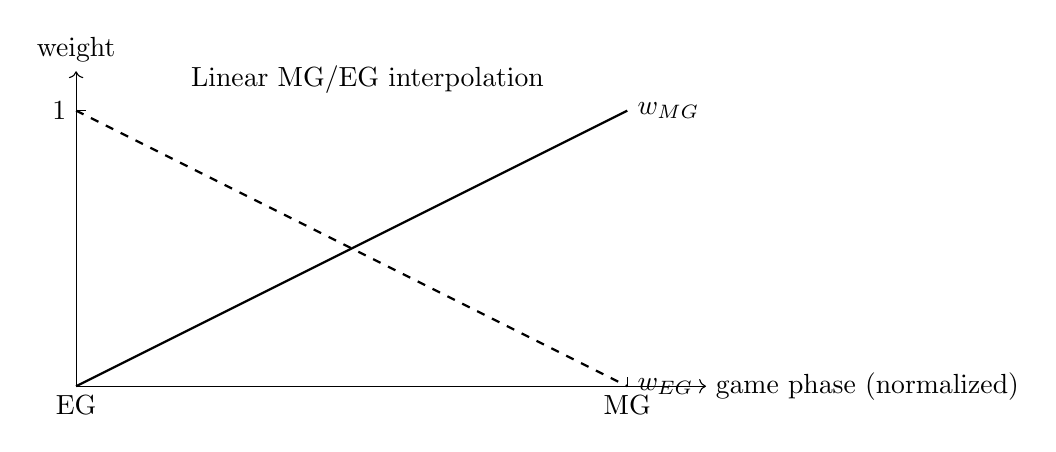
\begin{tikzpicture}[scale=1.0]
  \draw[->] (0,0) -- (8,0) node[right] {game phase (normalized)};
  \draw[->] (0,0) -- (0,4) node[above] {weight};

  % mg weight line: 0..1
  \draw[thick] (0,0) -- (7,3.5) node[right] {$w_{MG}$};
  % eg weight line: 1..0
  \draw[thick,dashed] (0,3.5) -- (7,0) node[right] {$w_{EG}$};

  % ticks
  \foreach \x/\lab in {0/EG,7/MG}{
    \draw (\x,0) -- (\x,0.12);
    \node[below] at (\x,0) {\lab};
  }
  \draw (0,3.5) -- (0.12,3.5);
  \node[left] at (0,3.5) {1};

  \node at (3.7,3.9) {Linear MG/EG interpolation};
\end{tikzpicture}
\caption{Tapered evaluation: midgame and endgame weights vary linearly with the
game phase.}
\label{fig:tapered_eval}
\end{figure}

\subsubsection{Tempo Bonus}
\label{subsec:tempo_bonus}

A constant tempo bonus is added to the final score to reflect the advantage of
having the next move. In the implementation, the returned evaluation is:
\[
Eval_\text{final}(P) = Eval(P) + 20.
\]
Since the engine evaluates positions from the perspective of the side to move,
this constant shifts the score slightly in favor of the player whose turn it is,
encouraging initiative and reducing symmetry artifacts.

\subsubsection{Algorithmic Summary}
\label{subsec:eval_algorithm}

\begin{algorithm}[ht]
\DontPrintSemicolon
\KwIn{Board position $P$}
\KwOut{Static evaluation score from the perspective of the side to move}

Initialize $mg[2]\gets 0$, $eg[2]\gets 0$, $phase\gets 0$\;

\For{$i \gets 0$ \KwTo $63$}{
    $piece \gets P[i]$\;
    $phase \gets phase + phaseValue(piece)$\;
    \uIf{$piece$ is white}{
        $idx \gets i \oplus 56$\tcp*{mirror for white}
        $mg[W] \gets mg[W] + MG\_PSQT(piece, idx) + MG\_MAT(piece)$\;
        $eg[W] \gets eg[W] + EG\_PSQT(piece, idx) + EG\_MAT(piece)$\;
    }
    \uElseIf{$piece$ is black}{
        $idx \gets i$\;
        $mg[B] \gets mg[B] + MG\_PSQT(piece, idx) + MG\_MAT(piece)$\;
        $eg[B] \gets eg[B] + EG\_PSQT(piece, idx) + EG\_MAT(piece)$\;
    }
}

$mgPhase \gets \min(24, phase)$\;
$egPhase \gets 24 - mgPhase$\;

Compute $MG(P)$ and $EG(P)$ as difference between side-to-move and opponent\;
$Eval(P) \gets \big(MG(P)\cdot mgPhase + EG(P)\cdot egPhase\big) / 24$\;

\Return $Eval(P) + 20$\tcp*{tempo}
\caption{Static evaluation with MG/EG separation, tapered interpolation, and tempo bonus.}
\label{algo:evaluation}
\end{algorithm}

\subsubsection{Limitations of the Evaluation}
\label{subsec:eval_limitations}

The evaluation is intentionally simple and focuses on material and PSQT-based
positional features. This makes it fast and easy to analyze, but it also implies
several limitations:
\begin{itemize}
    \item \textbf{Limited feature set:} Pawn structure (isolated/doubled/passed
    pawns), mobility, rook activity on open files, bishop pair, and advanced king
    safety concepts are not modeled explicitly.
    \item \textbf{No explicit drawishness detection:} The evaluation does not
    implement specialized scaling for fortress-like positions, opposite-coloured
    bishop endgames, or other draw-prone material configurations.
    \item \textbf{Constant tempo term:} The tempo bonus is a fixed constant and
    does not depend on phase or position characteristics.
    \item \textbf{No incremental evaluation:} The score is computed by scanning
    all 64 squares, rather than updating evaluation terms incrementally during
    make/unmake.
\end{itemize}

Despite these limitations, the evaluation is sufficient for the primary focus of
this thesis, namely the investigation of search behavior and iterative deepening
under time constraints. A stronger evaluation can be integrated later without
changing the surrounding search architecture.


\cleardoublepage
\section{Experimental Evaluation}
\label{sec:evaluation}

This section presents the experimental evaluation of the implemented chess
engine. The evaluation pursues the central question of this thesis: where lies
the sweet spot between invested search time and decision quality, and how do the
individual search refinements shift this trade-off? The strongest empirical
effect is produced by null-move pruning, which is therefore examined in detail,
while the Principal Variation Search parameter sweep yields a deliberate null
result that is reported and explained rather than hidden. All measurements are
based on a common position suite and a uniform scoring methodology, so that the
individual experiments remain directly comparable.

\subsection{Research Objectives}
\label{subsec:research_objectives}

The experimental evaluation addresses the following research questions:

\begin{itemize}
    \item \textbf{Playing strength:} how strong is the engine under realistic
    tournament time controls when compared to a fixed reference opponent?
    \item \textbf{Null-move pruning:} how does null-move pruning affect reachable
    depth, node throughput, transposition table behavior, and move quality across
    time budgets?
    \item \textbf{Transposition table size:} from which table size onward does
    the available memory stop limiting the search?
    \item \textbf{Time-to-quality and depth-versus-time:} how do reachable depth
    and move quality develop as the time budget increases, and where does
    additional time stop paying off?
    \item \textbf{PVS parameter sweep:} which combination of minimum scouting
    depth (\texttt{PvsMinDepth}) and number of fully searched moves
    (\texttt{PvsScoutAfterMove}) yields the best ratio of cost reduction to move
    quality?
    \item \textbf{Search tree reuse:} how much depth does a persistent
    transposition table gain over the course of a game compared to starting each
    search from an empty table?
    \item \textbf{Move stability:} at which search depth does the best move
    stabilize, so that deeper search no longer changes the decision?
\end{itemize}

The playing-strength question establishes an absolute reference point, while the
remaining questions characterize time-dependent decision making directly and
quantify the effect of the individual search refinements.

\subsection{Experimental Setup}
\label{subsec:common_setup}

Unless stated otherwise, all experiments share the following configuration.

\paragraph{Hardware and Build.}
All measurements were conducted on a MacBook Pro with an Apple M3 Pro processor
and 18\,GB of RAM. The engine was compiled in release mode and executed as a
single-threaded process. Apart from the parameter that is varied in a given
experiment, all engine options were kept at their defaults throughout.

\paragraph{Position Suite.}
The experiments use a fixed suite of 309 positions
(\texttt{tests/data/stockfish-bench-all.epd}), derived from the position set that
Stockfish uses for its own benchmark. Each configuration is measured with three
repetitions per position to average out scheduling noise, and reported figures
are means over positions and repetitions.

\paragraph{Time Budgets.}
Time-dependent experiments sweep a fixed set of per-move budgets of
$10, 25, 50, 100, 250, 500, 1000, 2000$, and $5000$\,ms. This range spans from
very short thinking times, where only shallow searches are possible, to budgets
that reach depths well into the middlegame.

\paragraph{Quality Scoring.}
Because the positions have no known ground-truth best move, move quality is
measured against a strong reference. For every position, Stockfish is run to a
fixed depth of 20 to obtain both a reference best move and a reference
evaluation. Two metrics are derived from this reference:
\begin{itemize}
    \item \textbf{Centipawn loss (CPL):} the difference, in centipawns and from
    the perspective of the side to move, between the reference evaluation of
    Stockfish's preferred move and the reference evaluation of the move actually
    played by the engine. Lower is better; a value of $0$ means the engine played
    a move of equal reference value.
    \item \textbf{Agreement:} the fraction of positions in which the engine's
    chosen move coincides exactly with Stockfish's reference move.
\end{itemize}
CPL is the primary quality metric, as it also credits moves that differ from the
reference move but are of comparable value; agreement is reported as a
complementary, stricter indicator.

\paragraph{Benchmark Harness.}
All experiments are driven by the dedicated benchmarking harness in the
\texttt{bench/} directory, which records for each search, among others, the
completed depth, selective depth, node and quiescence-node counts, the number of
PVS re-searches and null-move cutoffs, transposition table statistics, and the
elapsed time. The raw per-search records are written to CSV files and aggregated
offline, which keeps measurement and analysis reproducible. Each file also stores
the commit hash of the engine it was produced with, so every table in this
chapter can be traced back to a specific state of the implementation.

\paragraph{Correctness of the Move Generator.}
All results rest on the assumption that the engine generates and applies moves
correctly. This is verified with \emph{perft}~\cite{cpw_perft}, the standard
correctness test for
chess engines: for a set of reference positions, the number of leaf nodes of the
full game tree is counted up to a fixed depth and compared against published
values. Any error in move generation, in make--unmake, or in the handling of
castling, en-passant and promotion changes these counts and is thus detected. The
engine reproduces the reference values for all tested positions and depths.

\subsection{Playing Strength (Engine versus Engine)}
\label{subsec:engine_eval}

To place the engine on an absolute strength scale, it is evaluated in
head-to-head matches against a fixed reference opponent under tournament
conditions. The matches are played through the CuteChess framework, with a
development build of Stockfish as the reference opponent. To obtain a comparison
in the target strength range, Stockfish is restricted through its built-in
strength limitation (\texttt{UCI\_LimitStrength} with a nominal target of
2000\,Elo), a single search thread, and a 32\,MB hash; Helix likewise runs
single-threaded with a 32\,MB hash and otherwise default settings. Both engines
play a classical time control of five minutes per side with a 0.5\,second
increment.

To obtain a fair and diverse sample, the games are opened from a balanced opening
book (\texttt{8moves\_v3}), with each opening played once from either side so
that both engines receive identical starting positions as White and Black. In
total 400 games are played with alternating colors. Clearly decided games are
adjudicated to keep the match tractable: a game is scored as won once both
engines agree on an evaluation beyond $\pm 600$ centipawns for several
consecutive moves, and as drawn once the evaluation stays within $\pm 10$
centipawns for several moves in the late middlegame. All games run on the Apple
M3 Pro machine described in \cref{subsec:common_setup}. Playing strength is
reported as an Elo difference derived from the match result, together with the
likelihood of superiority (LOS) and the draw ratio.

\cref{tab:elo_results} summarizes the match.

\begin{table}[ht]
\centering
\begin{tabular}{@{}lr@{}}
\toprule
Metric & Value \\ \midrule
Games played & 400 \\
Score (W--L--D) & 288--76--36 \\
Elo difference & $+205.0 \pm 37.8$ \\
Likelihood of superiority & $100.0\,\%$ \\
Draw ratio & $9.0\,\%$ \\ \bottomrule
\end{tabular}
\caption{Match result of Helix against Stockfish limited to a nominal 2000\,Elo,
over 400 games at a 5+0.5 time control.}
\label{tab:elo_results}
\end{table}

Helix wins the match decisively, with an Elo difference of roughly $+205$ points
and a likelihood of superiority of $100\,\%$. The advantage holds with both
colors: Helix scores $138$--$40$--$22$ as White ($74.5\,\%$) and
$150$--$36$--$14$ as Black ($78.5\,\%$), so it remains clearly stronger even
without the first-move advantage. The moderate draw ratio of $9.0\,\%$ indicates
that most games are decided rather than drawn.

It should be emphasized that this is a \emph{relative} result. The reference
engine was deliberately weakened, and Stockfish's \texttt{UCI\_LimitStrength}
provides only a nominal Elo target that does not map directly onto established
rating lists; it also weakens play partly by introducing random inaccuracies
rather than uniformly. The reported difference therefore characterizes Helix's
strength relative to this specific, equally configured opponent, not an absolute
rating.

\subsection{Effect of Null-Move Pruning}
\label{subsec:eval_nmp}

Null-move pruning (\cref{subsec:null_move_pruning}) is the search refinement with
the largest measured effect on the engine. It was evaluated by running the full
time-budget sweep twice, once with pruning enabled and once disabled, on the
common suite. \cref{tab:nmp_depth_cpl} reports the reachable depth and the
centipawn loss for both configurations.

\begin{table}[ht]
\centering
\begin{tabular}{@{}rcccc@{}}
\toprule
 & \multicolumn{2}{c}{Completed depth (ply)} & \multicolumn{2}{c}{Centipawn loss} \\
\cmidrule(lr){2-3}\cmidrule(lr){4-5}
Budget (ms) & without NMP & with NMP & without NMP & with NMP \\ \midrule
10   & 3.67 & 3.91 & 60.2 & 61.9 \\
25   & 4.29 & 4.65 & 58.9 & 60.7 \\
50   & 4.86 & 5.30 & 57.1 & 56.0 \\
100  & 5.37 & 5.96 & 57.2 & 60.2 \\
250  & 6.04 & 6.81 & 54.6 & 55.7 \\
500  & 6.52 & 7.53 & 56.8 & 55.0 \\
1000 & 7.08 & 8.16 & 55.5 & 52.4 \\
2000 & 7.55 & 8.79 & 49.2 & 50.3 \\
5000 & 8.09 & 9.43 & 43.8 & 44.4 \\ \bottomrule
\end{tabular}
\caption{Reachable depth and centipawn loss with and without null-move pruning,
averaged over 309 positions and three repetitions per budget.}
\label{tab:nmp_depth_cpl}
\end{table}

The clearest and most robust effect is on search depth: null-move pruning reaches
a greater depth at \emph{every} one of the nine budgets, and the gap widens with
more time, from $+0.24$\,ply at 10\,ms to a full ply ($8.16$ versus $7.08$) at one
second and $+1.34$\,ply at five seconds. This confirms that skipping provably
weak subtrees lets the engine invest the saved effort into depth.

This additional depth is not bought at the cost of node throughput. At the
one-second budget the engine reaches about $1.69$ million nodes per second with
pruning versus $1.61$ million without, so pruning is if anything slightly faster
per node as well. What does change is the transposition table hit rate, which
drops from $0.208$ to $0.158$ at one second: by pruning subtrees, the search
visits a larger number of \emph{distinct} positions and re-visits known entries
less often. The hit rate is therefore best read as a symptom of the search shape
rather than as a quality target in itself.

The effect on move quality, however, does not follow the depth gain, and this is
reported here without smoothing. Across the nine budgets the pruning
configuration achieves a lower centipawn loss in only three cases (50\,ms,
500\,ms and 1000\,ms) and a higher one in the remaining six; averaged over all
budgets the difference amounts to $+0.37$\,cp in favour of the configuration
\emph{without} pruning, which is well inside the noise of three repetitions. The
largest single gain for pruning occurs at one second ($52.4$ versus $55.5$\,cp),
the largest loss at 100\,ms ($60.2$ versus $57.2$\,cp).

Taken together, this is the central and somewhat sobering observation of this
experiment: null-move pruning reliably buys depth, but the additional depth does
not translate into measurably better moves. A full extra ply at one second leaves
move quality statistically unchanged. This is the first direct piece of evidence
for the thesis question, and it is examined further in
\cref{subsec:eval_ttq,subsec:eval_move_stability}: beyond a certain point the
engine is not limited by how deep it searches, but by what its evaluation can
distinguish. \cref{fig:quality_vs_depth,fig:search_nps} visualize the quality and
the node throughput across budgets.

\begin{figure}[ht]
\centering
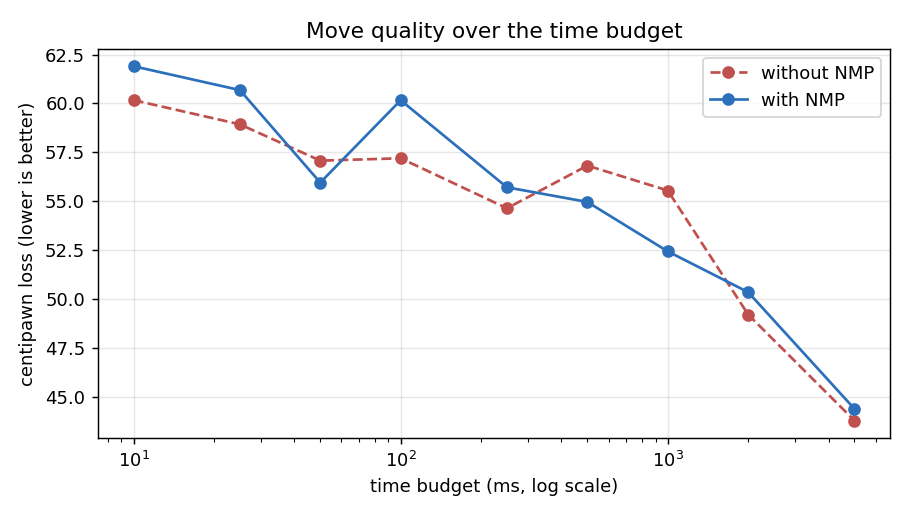
\includegraphics[width=0.8\linewidth]{figures/quality_vs_depth.png}
\caption{Centipawn loss as a function of the reached depth (and thus time budget)
with and without null-move pruning.}
\label{fig:quality_vs_depth}
\end{figure}

\begin{figure}[ht]
\centering
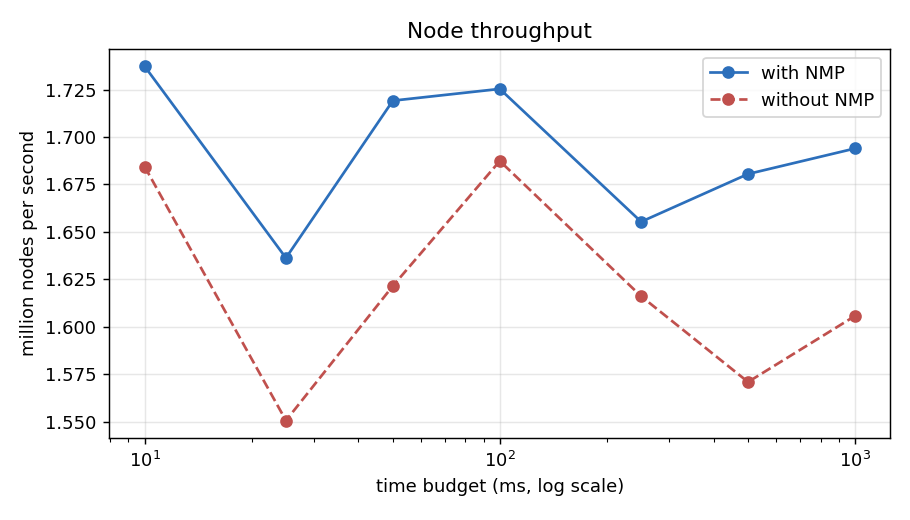
\includegraphics[width=0.8\linewidth]{figures/search_nps.png}
\caption{Node throughput (nodes per second) across time budgets with and without
null-move pruning.}
\label{fig:search_nps}
\end{figure}

\subsection{Transposition Table Size}
\label{subsec:eval_tt_size}

The transposition table trades memory for search efficiency: a larger table
retains more previously computed positions but consumes more memory. To determine
a sensible default, the table size was swept over $1, 4, 16, 64$, and $256$\,MB
at a fixed one-second budget, with null-move pruning enabled.
\cref{tab:tt_size} reports the reachable depth, the eviction rate (the share of
stores that overwrite an entry of a different position), and the hit rate.

\begin{table}[ht]
\centering
\begin{tabular}{@{}rccc@{}}
\toprule
Table size (MB) & Completed depth (ply) & Eviction rate & Hit rate \\ \midrule
1   & 7.75 & 0.610 & 0.104 \\
4   & 8.01 & 0.263 & 0.134 \\
16  & 8.14 & 0.076 & 0.153 \\
64  & 8.18 & 0.019 & 0.161 \\
256 & 8.18 & 0.005 & 0.163 \\ \bottomrule
\end{tabular}
\caption{Effect of transposition table size at a one-second budget, averaged over
309 positions and three repetitions.}
\label{tab:tt_size}
\end{table}

Only the smallest table has a measurable negative effect: at 1\,MB the search
loses roughly half a ply of depth ($7.75$ versus $\approx 8.2$) while more than
$60\,\%$ of all stores evict a foreign entry, so useful information is displaced
before it can be reused. From 16\,MB onward the curve flattens; the difference
between 64\,MB and 256\,MB is within noise, even though the eviction rate keeps
falling. For the target time controls the search therefore stops being
memory-bound well below 32\,MB, which justifies the default hash size used
elsewhere in this work.

\subsection{Time-to-Quality and Depth-versus-Time}
\label{subsec:eval_ttq}

The per-budget measurements in \cref{tab:nmp_depth_cpl} also answer the
time-to-quality and depth-versus-time questions directly. Reachable depth grows
smoothly and predictably with the budget, roughly one additional ply per
doubling of time in the tested range, which reflects the exponential relationship
between depth and node count discussed in \cref{sec:preliminaries}.

Move quality, in contrast, improves far less smoothly. Over the whole range from
10\,ms to 5000\,ms, a factor of 500 in thinking time, the centipawn loss of the
pruning configuration falls only from about $62$ to $44$\,cp, and it does so
non-monotonically: the curve rises again at 100\,ms and at 2000\,ms before
continuing downwards. Put differently, the first $250$\,ms buy roughly three
plies of depth but barely six centipawns of quality, while the last step from
2000 to 5000\,ms buys a further $0.6$\,ply and six more centipawns.

This is the central observation behind the thesis question. Depth and decision
quality are not proportional: additional search time reliably converts into
depth, but only weakly into better moves. The engine typically finds a move of
comparable quality early and spends the remaining time confirming it, which is
consistent with the move stability results in
\cref{subsec:eval_move_stability}. The practical sweet spot therefore lies where
the depth curve is still rising steeply while the quality curve has already
flattened, which for this engine and suite is reached around one second per move.

\subsection{Distribution of Move Quality}
\label{subsec:eval_outliers}

All centipawn losses reported so far are means over the suite, and that summary
turns out to hide the actual behavior of the engine. The distribution of the
per-position loss is strongly skewed: at a one-second budget the \emph{median}
loss is $2$\,cp while the \emph{mean} is $52.4$\,cp. In $49.0\,\%$ of all
positions the engine plays exactly the move Stockfish prefers, and in $66.3\,\%$
it stays within $25$\,cp of it. At the other end, $6.9\,\%$ of the positions
(21 of 306) exceed $200$\,cp, and the fifteen worst positions alone account for
$46.3\,\%$ of the entire mean. The average is therefore not a description of the
typical case, it is a description of a small number of failures.

This also changes how the time-to-quality result of \cref{subsec:eval_ttq} should
be read. Measured by the median, additional time helps clearly and monotonically:
the median loss falls from $16$\,cp at 10\,ms over $7$\,cp at 100\,ms to $2$\,cp
at one second. The mean, dominated by the outliers, barely moves over the same
range. The engine does not gradually get better at every position, it solves more
and more positions outright while a hard residue stays unsolved regardless of the
budget.

The outliers share a recognizable profile. Positions with a loss above $200$\,cp
hold on average $13.8$ pieces, against $19.5$ for the well-played ones, and a
third of them are endgames with ten pieces or fewer. Three positions reach the
scoring cap of $1000$\,cp, meaning Stockfish sees a forced mate the engine misses
entirely. A typical example is the pawn endgame
\texttt{8/1p3pp1/7p/5P1P/2k3P1/8/2K2P2/8 w}, in which the engine plays
\texttt{g4g5} instead of the winning \texttt{f5f6}.

This is a direct consequence of the evaluation function discussed in
\cref{subsec:eval_limitations}. Material and piece-square tables describe a
middlegame reasonably well, but they encode nothing about passed pawns,
opposition or king activity, the very concepts that decide sparse endgames. In
such positions no attainable search depth compensates for what the evaluation
cannot express, which is consistent with these positions being exactly the ones
that never stabilize in \cref{subsec:eval_move_stability}. It also explains why
the depth gained through null-move pruning does not show up in the mean: the
positions where extra depth would matter are the ones limited by evaluation
knowledge, not by depth.

\subsection{PVS Parameter Sweep}
\label{subsec:eval_pvs_sweep}

Principal Variation Search exposes two tunable parameters, the minimum scouting
depth (\texttt{PvsMinDepth}) and the number of leading moves searched with the
full window (\texttt{PvsScoutAfterMove}). To determine whether these parameters
offer a worthwhile tuning gain, a full grid of $6 \times 5 = 30$ configurations
(\texttt{PvsMinDepth} $1$ to $6$, \texttt{PvsScoutAfterMove} $1$ to $5$) was
evaluated on the full suite at a one-second budget with null-move pruning
enabled. \cref{tab:pvs_sweep} lists a representative selection.

\begin{table}[ht]
\centering
\begin{tabular}{@{}ccccc@{}}
\toprule
\texttt{PvsMinDepth} & \texttt{PvsScoutAfterMove} & Depth (ply) & Nodes & Re-searches \\ \midrule
1 & 1 & 8.16 & 1\,534\,720 & 104.1 \\
2 & 1 & 8.15 & 1\,531\,145 & 52.2 \\
3 & 1 & 8.16 & 1\,539\,544 & 29.2 \\
6 & 5 & 8.09 & 1\,531\,458 & 3.2 \\ \bottomrule
\end{tabular}
\caption{Representative configurations from the PVS parameter sweep (one-second
budget). The default configuration is \texttt{PvsMinDepth}\,$=2$,
\texttt{PvsScoutAfterMove}\,$=1$.}
\label{tab:pvs_sweep}
\end{table}

The sweep is a deliberate null result: across all 30 configurations the completed
depth stays between $8.09$ and $8.16$\,ply and the node count between $1.52$ and
$1.55$ million, a spread of about $1.8\,\%$ that is within measurement noise. No
configuration offers a meaningful improvement over any other.

The reason is visible in the re-search column. The whole point of the scouting
parameters is to control the trade-off between the savings of the cheap
null-window scout and the cost of the occasional full-window re-search when the
scout fails high. In this engine that trade-off barely materializes: even the
most aggressive configuration triggers only about $104$ re-searches over roughly
$1.5$ million nodes, and the most conservative one only about $3$. The existing
move ordering (transposition-table move, MVV-LVA captures, killer moves, and the
history heuristic) is already good enough that the first move is almost always
the best, so the null-window scout almost always holds and there is little
re-search cost left for the parameters to tune away. As a side observation, the
transposition table hit rate correlates weakly with the number of re-searches
($0.158$ at $104$ re-searches versus $0.144$ at $3$), which again confirms that
the hit rate reflects the shape of the search rather than being an independent
quality target. Consequently, the default configuration
(\texttt{PvsMinDepth}\,$=2$, \texttt{PvsScoutAfterMove}\,$=1$) is retained, as no
setting in the sweep improves upon it.

\subsection{Search Tree Reuse}
\label{subsec:eval_tree_reuse}

The second refinement of this thesis is the reuse of previously explored search
trees through a persistent transposition table (\cref{subsec:tree_reuse}). Its
value cannot be measured on isolated positions, since it only materializes when
consecutive searches are related, so this experiment replays complete games
instead. The 30 games are taken from the match of \cref{subsec:engine_eval}, and
every position of every game is searched with a fixed budget of 500\,ms, once in
each of two modes: in \emph{keep} the table survives the whole game, which is the
engine's normal behavior, and in \emph{clear} it is wiped before every single
search. Both runs see identical positions under identical budgets, so the
difference between them is precisely the value of resuming the old tree.
\cref{tab:tree_reuse} reports the aggregate over all 2256 plies.

\begin{table}[ht]
\centering
\begin{tabular}{@{}lccc@{}}
\toprule
Mode & Completed depth (ply) & TT hit rate & Nodes \\ \midrule
TT cleared each move & 7.23 & 0.136 & 758\,979 \\
TT kept (tree reuse) & 7.52 & 0.152 & 772\,368 \\ \bottomrule
\end{tabular}
\caption{Effect of search tree reuse over 30 complete games (2256 plies) at a
500\,ms budget per move.}
\label{tab:tree_reuse}
\end{table}

Keeping the table yields $+0.28$\,ply on average at an unchanged time budget,
together with a hit rate that rises from $0.136$ to $0.152$, i.e., by about
$12\,\%$ relative. A paired comparison per position shows how this average comes
about: in $69\,\%$ of all plies both modes reach exactly the same depth, in
$28\,\%$ the persistent table reaches deeper, and only in the remaining few does
the cleared table win. Tree reuse thus does not speed up every single search, it
provides a head start in those positions where the new root actually lies inside
the previously explored tree.

That reading is supported by the development over the course of a game, shown in
\cref{fig:tree_reuse}. The gain grows from $+0.16$\,ply in the opening
(plies 0--15) over $+0.22$ in the middlegame to $+0.39$ in the endgame
(ply 41 onwards), where the hit rate also climbs to $0.207$ versus $0.178$. With
fewer pieces on the board, positions transpose more often and a larger share of
the stored tree remains reachable, so the retained information keeps paying off
increasingly as the game progresses.

\begin{figure}[ht]
\centering
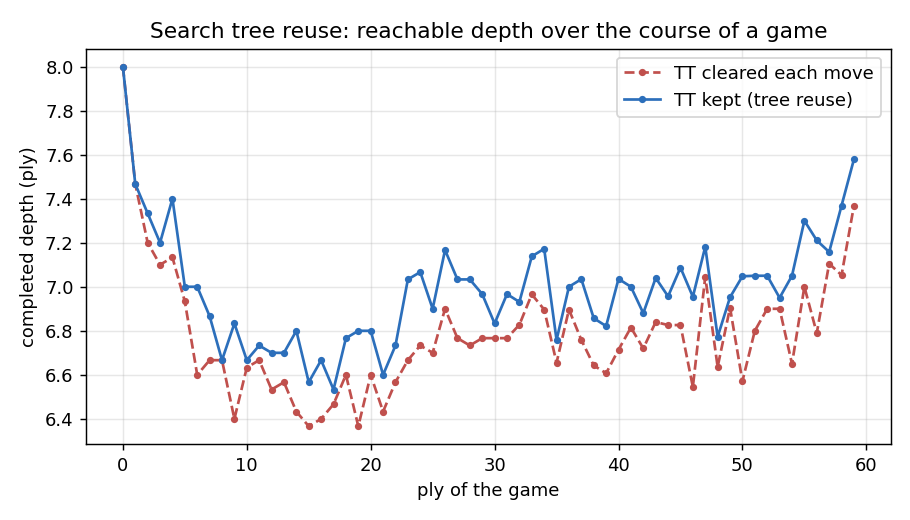
\includegraphics[width=0.8\linewidth]{figures/tree_reuse.png}
\caption{Reachable depth per ply of the game, averaged over 30 games, with the
transposition table kept versus cleared before every search.}
\label{fig:tree_reuse}
\end{figure}

Compared to null-move pruning, the effect is smaller in absolute terms ($+0.28$
versus a full ply), but it comes at no cost whatsoever: no search parameter is
changed, nothing is pruned away, and no accuracy is traded. The engine merely
stops discarding what it has already computed.

\subsection{Move Stability}
\label{subsec:eval_move_stability}

The final question concerns move stability: at which depth does the engine's
chosen move settle, so that deeper search no longer changes the root decision?
This is measured with a single iterative-deepening search per position. Because
iterative deepening already produces a best move at every completed depth, one
search yields the full sequence of root moves without repeated re-searching. Each
position is searched under a fixed budget of 20 million nodes with the
transposition table cleared beforehand, so that the depth sequence reflects one
self-contained search. A node budget is used instead of a fixed target depth
because it bounds the cost per position and, being independent of wall-clock time,
is unaffected by other load on the machine.

For each position the \emph{stabilization depth} is defined as the smallest depth
from which the root move matches the move of the deepest completed iteration and
does not change again \emph{within the searched range}. Positions whose move still
changes at the deepest searched depth are counted as not yet settled within the
budget. Of the 309 positions, 306 produced a usable move sequence, reaching a mean
depth of $10.1$ plies. \cref{fig:move_stability} shows the cumulative distribution
and \cref{tab:move_stability} lists selected thresholds.

This definition can only observe what happens inside the budget, which has to be
kept in mind when reading the numbers. A move that survives until the last
completed iteration might still change one ply deeper, and the evidence for a late
stabilization is necessarily thinner than for an early one: a position that
settles at depth 3 and is searched to depth 11 confirms that move eight more
times, whereas one that settles at depth 10 out of 11 confirms it once. The
measurement quantifies this directly. On average a stabilized move is confirmed by
$4.3$ further iterations (median 3), but for $22.2\,\%$ of the positions the move
changed in the very last iteration, which is why those are reported as unsettled
rather than as stabilized at the final depth. Restricting the analysis to the 178
positions whose move is confirmed by at least three further iterations shifts the
median stabilization depth down to 3 plies, with $87\,\%$ settled by depth 6.
That subset is itself selective, since it excludes late stabilizers by
construction, so the two views bracket the effect rather than replacing one
another: the reported figures are an upper bound on the depth actually needed.

\begin{figure}[ht]
\centering
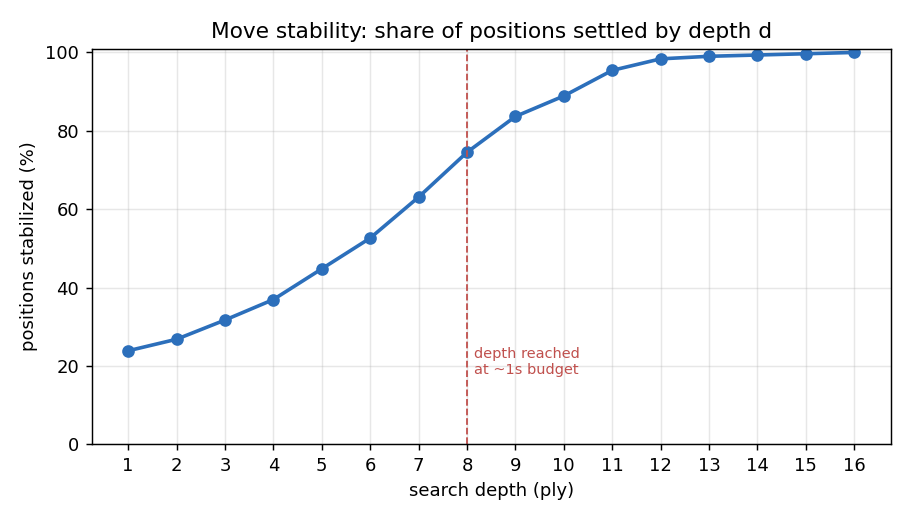
\includegraphics[width=0.8\linewidth]{figures/move_stability.png}
\caption{Share of positions whose root move is settled by depth $d$. The dashed
vertical line marks the depth ($\approx 8$) the engine reaches at a one-second
budget.}
\label{fig:move_stability}
\end{figure}

\begin{table}[ht]
\centering
\begin{tabular}{@{}rr@{}}
\toprule
Depth $d$ (ply) & Positions settled by $d$ \\ \midrule
2  & $26.8\,\%$ \\
4  & $36.9\,\%$ \\
6  & $52.6\,\%$ \\
8  & $74.5\,\%$ \\
10 & $88.9\,\%$ \\ \bottomrule
\end{tabular}
\caption{Cumulative share of positions whose best move has stabilized by a given
depth (306 positions, 20-million-node budget).}
\label{tab:move_stability}
\end{table}

The root move settles early for most positions: the median stabilization depth is
6 plies, and $23.9\,\%$ of positions never change their move at all. By depth 8,
roughly the depth the engine reaches at a one-second budget
(\cref{tab:nmp_depth_cpl}), three quarters of all positions have already locked in
their final move. This is the central evidence for the sweet-spot argument of this
thesis: beyond this point additional search keeps increasing depth but only rarely
changes the decision.

At the same time, the effect is not uniform. Roughly one position in five
($22.2\,\%$) still changes its move at the deepest depth searched, i.e., remains
unsettled even around depth 10 and beyond. These are the tactically sharp
positions in which deeper search still changes the decision, and they are the
only ones for which the extra ply bought by null-move pruning
(\cref{subsec:eval_nmp}) can pay off at all. Since they make up only a fifth of
the suite, an across-the-board gain in depth is diluted accordingly, which
explains why the substantial depth gain of null-move pruning leaves the average
centipawn loss unchanged. Move stability is therefore concentrated: the majority of decisions are
made cheaply and early, while a hard minority keeps rewarding deeper search.

\subsubsection{Stability in Evaluation Rather Than in the Move}
\label{subsubsec:eval_eps_stability}

Judging stability by the identity of the move has a blind spot: a switch between
two moves of equal value counts as instability, while converging on a
consistently poor move counts as success. To separate these cases, every move of
every iteration was additionally scored against the reference engine, and a
position is called \emph{$\varepsilon$-stable} from the smallest depth at which
its centipawn loss stays below $\varepsilon$ for all deeper iterations.
\cref{tab:eps_stability} contrasts the two criteria and \cref{fig:eps_stability}
shows the corresponding curves.

\begin{table}[ht]
\centering
\begin{tabular}{@{}lcccc@{}}
\toprule
Criterion & Positions reaching it & Median depth & By depth 6 & By depth 8 \\ \midrule
Move identity            & $100\,\%$  & 6 & $52.5\,\%$ & $74.4\,\%$ \\
$\varepsilon = 0$\,cp    & $52.5\,\%$ & 4 & $35.1\,\%$ & $43.9\,\%$ \\
$\varepsilon = 20$\,cp   & $66.9\,\%$ & 2 & $49.5\,\%$ & $60.0\,\%$ \\
$\varepsilon = 50$\,cp   & $78.4\,\%$ & 1 & $63.6\,\%$ & $72.1\,\%$ \\ \bottomrule
\end{tabular}
\caption{Move stability judged by move identity versus by evaluation, for 305
scored positions. Percentages refer to the whole set, so positions that never
reach the criterion are included in the denominator.}
\label{tab:eps_stability}
\end{table}

\begin{figure}[ht]
\centering
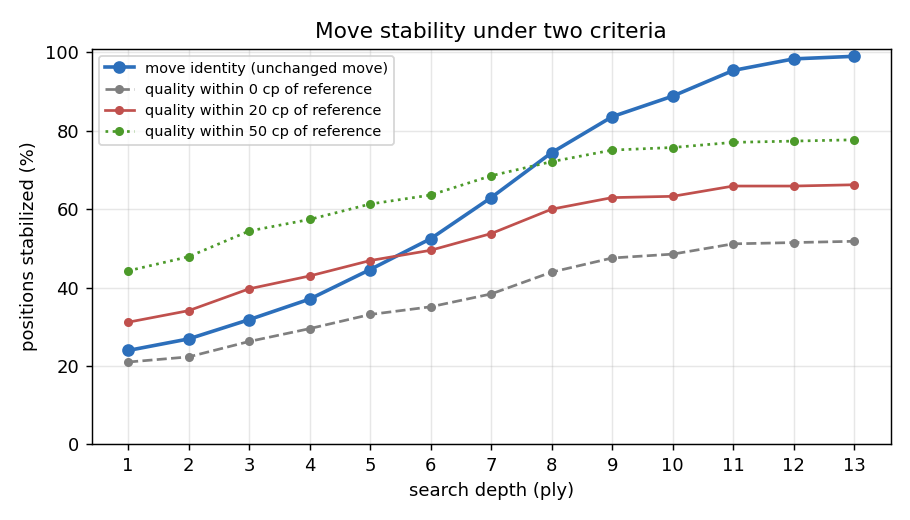
\includegraphics[width=0.8\linewidth]{figures/move_stability_eps.png}
\caption{Cumulative share of positions considered stable by depth $d$, judged by
the identity of the move and by its distance to the reference evaluation.}
\label{fig:eps_stability}
\end{figure}

The two criteria disagree in both directions, and the curves cross at around
depth 6. Below that, judging by evaluation reports \emph{more} stability: at
depth 3 already $39.7\,\%$ of the positions are within 20\,cp, against $31.8\,\%$
whose move has settled. The engine reaches a decision of adequate quality earlier
than it settles on one particular move, since part of the apparent instability is
merely alternation between moves of comparable value.

Above depth 6 the relation reverses, and this is the more consequential half. By
move identity, $88.9\,\%$ of the positions have settled by depth 10; measured
against the reference evaluation, only $63.3\,\%$ are within 20\,cp, and
$33.1\,\%$ never reach that margin at any depth. These are not positions in which
the move keeps changing: their move does settle, but it settles on something
poor, with a mean loss of $120$\,cp at the deepest iteration. Fourteen of the 21
worst positions from \cref{subsec:eval_outliers} are among them.

Both readings therefore support the same conclusion from opposite sides. Where
the engine is able to find a good move, it finds it early, earlier than the
move-identity criterion suggests. Where it is not, the search converges
confidently on the wrong answer. Stability of the move is thus a necessary but
not a sufficient indicator of a settled decision.

It is worth asking whether these positions would simply need more depth. The data
argue against it. Both groups are searched to the same average depth of $10.1$
plies under the shared node budget, so the difference is not one of search effort.
What differs is how much that effort achieves: comparing the first half of each
search to the second, and excluding the final iteration that defines the grouping,
the loss falls by $36.5$\,cp on average for the positions that do converge, but
only by $5.4$\,cp for those that do not. The same picture emerges when comparing
shallow to intermediate depths, where the converging positions gain $41.5$\,cp and
the others $21.9$\,cp. Additional depth is therefore not without effect on the
difficult positions, but it is roughly half to one seventh as effective, and it
starts from a worse level. Extrapolating the observed rate, the remaining gap of
over $100$\,cp would not be closed by the few plies that are realistically
attainable. The bottleneck lies in the evaluation, which cannot express what
distinguishes these positions, and a search that optimizes a misleading objective
more thoroughly does not arrive at a better move.


\cleardoublepage
\section{Conclusions and Future Work}
\label{sec:discussion}

The experiments of \cref{sec:evaluation} allow the central question of this
thesis to be answered, and the answer is more nuanced than the initial
formulation suggested. This section relates the individual results to that
question, draws the overall conclusions, and outlines where the engine would have
to be extended for the remaining gap to close.

\subsection{Depth and Decision Quality Are Not Proportional}
\label{subsec:discussion_depth_vs_quality}

The clearest finding of this work is that additional search depth does not
translate into proportionally better decisions. Null-move pruning
(\cref{subsec:eval_nmp}) reaches a greater depth at every single one of the nine
time budgets, at one second a full ply, and yet the mean centipawn loss remains
statistically unchanged. Search tree reuse (\cref{subsec:eval_tree_reuse}) adds
another $0.28$ ply at no cost at all. Both refinements do exactly what they are
designed to do, and neither shows up as a measurable gain in move quality on the
test suite.

The move stability measurements (\cref{subsec:eval_move_stability}) explain why.
By depth 8, the depth the engine reaches at a one-second budget, three quarters
of all positions have already settled on their final move, and about a quarter
never change it from the very first iteration. Deeper search can only change the
decision in the remaining fifth of positions, so an across-the-board gain in
depth is diluted accordingly. This is the practical sweet spot the thesis asked
for: it lies where the depth curve is still rising while the quality curve has
already flattened, for this engine and suite at roughly one second per move.

\subsection{Where the Search Is Actually Limited}
\label{subsec:discussion_limits}

The distribution of move quality (\cref{subsec:eval_outliers}) shows where the
remaining errors come from. The engine plays exactly Stockfish's move in
$49\,\%$ of the positions and stays within $25$\,cp in two thirds of them, with a
median loss of $2$\,cp. The mean of $52$\,cp is produced almost entirely by a
small residue: fifteen positions account for nearly half of it.

These positions share a profile. They hold fewer pieces than average, a third of
them are endgames, and three contain a forced mate the engine does not find.
They are precisely the positions in which material and piece-square tables carry
no useful information, since passed pawns, opposition and king activity are not
represented in the evaluation (\cref{subsec:eval_limitations}). In such
positions the limiting factor is not how deep the engine searches but what its
evaluation is able to distinguish, and no attainable depth compensates for that.

Judging stability by evaluation instead of by the identity of the move makes the
consequence explicit (\cref{subsubsec:eval_eps_stability}). While the move
settles in nearly every position, a third of them never come within 20\,cp of the
reference at any depth, ending at an average loss of $120$\,cp. The search does
not remain undecided in these cases, it converges, and it converges on the wrong
move. A stable decision is therefore not by itself a good one, which is worth
keeping in mind wherever move stability is used as a stopping criterion in
time management.

That these positions are limited by evaluation rather than by depth can be shown
directly. They are searched just as deeply as the rest, to the same average of
$10.1$ plies, but they convert that depth into far less: over the course of a
search their loss improves by $5.4$\,cp where the converging positions gain
$36.5$\,cp. Depth is not useless there, it is merely too weak a lever to close a
gap of more than $100$\,cp. This is the clearest argument that further effort
belongs in the evaluation function: a search that optimizes a misleading
objective more thoroughly only becomes more certain of the wrong answer.

This also puts the null result of the parameter sweep
(\cref{subsec:eval_pvs_sweep}) into perspective. Across all 30 configurations the
node count varies by less than two percent, because re-searches are rare to begin
with: even the most aggressive scouting triggers about 104 of them over 1.5
million nodes. The move ordering, built from transposition table moves, MVV-LVA,
killer moves and the history heuristic, is already good enough that the first
move examined is almost always the best one. This is consistent with the
long-standing observation that the effectiveness of Alpha-Beta pruning is
governed by move ordering rather than by the pruning scheme
itself~\cite{knuth1975alphabeta, marsland1986review}, and it means the scouting
parameters have almost no trade-off left to tune.

\subsection{Implications for Time-Managed Search}
\label{subsec:discussion_time}

For iterative deepening under time constraints~\cite{korf1985iterative} these
results are encouraging. The anytime property is not merely a safety net: since
most positions settle early, an interrupted search usually returns the same move
a deeper one would have confirmed. Stopping between iterations therefore costs
far less quality than the depth difference alone would suggest.

The measurements also show that the engine stops being memory-bound well below
the default hash size (\cref{subsec:eval_tt_size}). Only the smallest table
degrades the search measurably, while beyond 16\,MB the curve flattens. Combined
with the tree reuse result, this argues for keeping the table alive across moves
rather than enlarging it: retaining what was already computed helps more than
providing space for more of it, and the benefit grows over the course of a game
as positions transpose more frequently~\cite{warnock1988search}.

Under tournament conditions all of this adds up to a clear result: the engine
wins its match against the reference opponent by roughly $205$ Elo points
(\cref{subsec:engine_eval}), with both colors and a low draw ratio.

\subsection{Limitations}
\label{subsec:discussion_limitations}

Several limitations qualify these conclusions. Move quality is measured against a
strong reference engine rather than against ground truth, so agreement with
Stockfish is treated as a proxy for correctness; positions in which a different
move is equally good are penalised by the agreement metric, which is why
centipawn loss is used as the primary measure.

The suite consists of 309 predefined positions with three repetitions each. It is
large enough for the aggregate effects reported here, but the skewed distribution
of the loss means that individual means are sensitive to a small number of
positions, and differences of a few centipawns should not be over-interpreted.

The opponent in the match was deliberately weakened through Stockfish's built-in
strength limitation. That mechanism provides only a nominal Elo target and works
partly by introducing random inaccuracies, so the reported difference describes
the relation to this specific configuration and not an absolute rating.

Finally, the engine uses a mailbox board representation and a handcrafted
evaluation, both chosen for clarity rather than for strength. Modern engines rely
on bitboards~\cite{cpw_bitboards} and learned evaluation
functions~\cite{silver2018alphazero}, and the conclusions about absolute playing
strength do not transfer to those designs.

\subsection{Future Work}
\label{subsec:discussion_future}

The results point to one clear priority. Since the residual errors are
concentrated in positions the evaluation cannot describe, further work should be
directed at the evaluation function rather than at the search. Pawn structure,
passed pawns, king activity and dedicated endgame knowledge would address exactly
the positions that dominate the mean loss today, and only then would the depth
already gained by null-move pruning and tree reuse have anything left to
contribute.

A second direction concerns the measurement itself. Reporting the median
alongside the mean, or trimming the extreme cases, would make the effect of
search refinements visible at all, since the mean is dominated by a residue that
no search improvement can fix.

The stability analysis could be extended in the same spirit. Judging convergence
by evaluation rather than by the identity of the move already proved more
informative here (\cref{subsubsec:eval_eps_stability}); applying the same
criterion to the time-to-quality measurements, and reporting from which
\emph{budget} rather than from which depth the loss stays within a margin, would
describe the practical behavior of the engine under a clock more directly than
the depth-based view can.

Finally, the search refinements evaluated here are only the beginning of what a
classical engine typically employs. Late move reductions, aspiration windows and
static exchange evaluation all target the same goal of spending effort where it
changes the decision, and the move ordering measured here is strong enough that
they would likely pay off.

\subsection{Summary}

This thesis implemented a complete chess engine and used it to examine how
invested search time translates into decision quality. Both refinements studied
work as intended: null-move pruning gains a full ply at one second, and a
persistent transposition table adds a further $0.28$ ply for free, growing to
$0.39$ ply in the endgame. Neither improves the average move quality measurably,
because three quarters of all positions have settled by the depth the engine
already reaches, and the remaining errors are concentrated in endgames that the
evaluation cannot assess regardless of depth.

The sweet spot between search time and decision quality is therefore reached
earlier than expected, at around one second per move for this engine. Beyond that
point, additional time keeps buying depth but no longer buys decisions. What
limits the engine at that stage is no longer how far it looks ahead, but what it
is able to recognise when it gets there.



\end{document}